\documentclass[10pt]{beamer}
\usetheme[progressbar=frametitle]{metropolis}

\usepackage{hyperref}
\usepackage{media9} 
\usepackage{appendixnumberbeamer}
\usepackage{minted}
\usemintedstyle{trac}
\usepackage{graphicx}
\graphicspath{{pictures/}}
\usepackage{mathtools,amsmath,amsfonts,amssymb}
\usepackage{xepersian}
\usepackage{fontspec}

\setminted{fontsize=\tiny}

\settextfont[
	Path=./fonts/,
	Extension=.ttf,
]{B Yas}

\setlatintextfont[
	Path=./fonts/,
	Extension=.ttf,
	UprightFont=Times New Roman,
]{Times New Roman}

\setmonofont[
	Path=./fonts/,
	Extension=.ttf,
	UprightFont=*-Regular,
	BoldFont=*-Bold,
	Ligatures=TeX,
]{Fira Code}

\setbeamertemplate{itemize item}{\color{black}$\bullet$}
\setbeamertemplate{itemize subitem}{\color{black}$\bullet$}
\title{الگوریتم \lr{ Fuzzy c-means}
و کاربرد آن در پردازش تصاویر
}
\subtitle{پیاده سازی، چالش ها و مقایسه با روش های دیگر}
\author{علیرضا عظیمی }
\date{ }

\begin{document}
	
\begin{frame}[plain]
		\maketitle
\end{frame}
	

\begin{frame}{فهرست مطالب}
	\setbeamertemplate{section in toc}[sections numbered]
	\tableofcontents[hideallsubsections]
\end{frame}

\begin{frame}{خوشه بندی }

\section{خوشه بندی \lr{ Clustering}}

خوشه بندی \lr{clustering} یک روش یادگیری ماشین بدون نظارت است که داده ها را بر اساس شباهت هایشان به گروه هایی (خوشه هایی) تقسیم می کند. بدون اینکه از قبل برچسب یا دسته بندی مشخصی صورت گرفته باشد، هدف یافتن الگو یا ساختار پنهان در داده هاست.

\textbf{چرا از خوشه بندی استفاده می کنیم؟}

\begin{itemize}
	\item 
کشف الگو های پنهان
	\item 
تحلیل داده ها
	\item 
کاهش پیچیدگی 
\end{itemize}

\end{frame}

	
\begin{frame}{انواع روش های خوشه بندی}
\begin{enumerate}
	\item{\textbf{خوشه بندی مبتنی بر مرکز \lr{ centroid-based}}}
	
\begin{footnotesize}
	در این نوع خوشه بندی داده به \lr{k} خوشه تقسیم شده، که هر خوشه دارای یک مرکز می باشد.
	
	مثل الگوریتم \lr{k-means} و \lr{Fuzzy c-means}
	
	کاربرد : ساده و سریع برای داده های عددی.
\end{footnotesize}
	\item{\textbf{خوشه بندی سلسله مراتبی \lr{ hierarchical}}}
	\begin{footnotesize}
		
		در این نوع خوشه بندی، خوشه ها به صورت درختی از پایین به بالا یا از بالا به پایین ساخته می شوند.
		
		کاربرد مناسب برای داده های کوچک و نمایش روابط سلسله مراتبی
		
	\end{footnotesize}
	\item{\textbf{ خوشه بندی مبتی بر چگالی\lr{ Density-based}}}
	\begin{footnotesize}

خوشه بندی بر اساس نقاط متراکم داده ها شکل می گیرد، مثل الگوریتم \lr{DB-scan}

کاربرد : شناسایی خوشه هایی با شکل های غیر منظم و حذف نویز

	\end{footnotesize}
			\item[4.]{\textbf{خوشه بندی مبتنی بر توزیع \lr{ }}}
			
		\begin{footnotesize}
		در این نوع خوشه بندی فرض می شود داده ها از توزیع های آماری خاص تولید شده اند مثل الگوریتم \lr{GMM} (مدل مخلوط گاوسی)

کاربرد: داده پیچیده با توزیع های آماری

		\end{footnotesize}
		\item[5.]{\textbf{ خوشه بندی مبتنی بر گراف\lr{ }}}
		
\begin{footnotesize}
		داده ها به صورت گراف مدل شده و خوشه ها بر اساس اتصالات گرافی شناسایی می شوند.

کاربرد : شبکه های اجتماعی 
\end{footnotesize}
	\end{enumerate}
\end{frame}
	
\begin{frame}{انواع روش های خوشه بندی}
	\begin{center}
		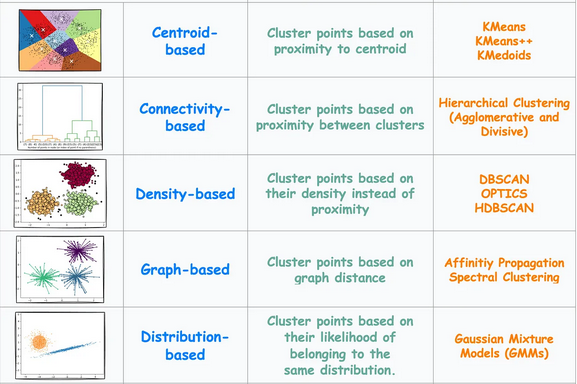
\includegraphics[height=8cm, width=10cm]{types_of_clustering}
	\end{center}
\end{frame}

\begin{frame}{\lr{k-means Algorithm}}
	\section{\lr{K-means Algorithm}}
الگوریتم \lr{k-means} برای اولین بار در سال 1967 توسط \lr{James Mac Queen} به کار گرفته شد.

ایده اصلی این الگوریتم از پردازش سیگنال گرفته شده و هدف آن تقسیم \lr{n} نقطه (داده) به \lr{k} خوشه است. در این الگوریتم هر داده متعلق به خوشه ای است که داده نزدیک ترین فاصله را با مرکز خوشه داشته باشد.
\end{frame}	

\begin{frame}{\lr{k-means Algorithm}}
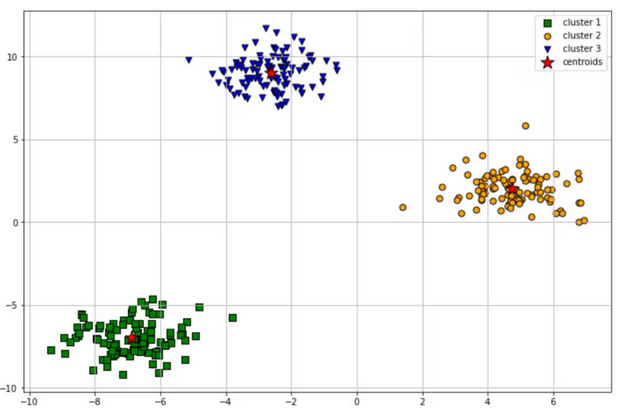
\includegraphics[height=8cm, width=10cm]{clustering}
\end{frame}

\begin{frame}{\lr{k-means Algorithm}}
\textbf{مزایا و معایب 
الگوریتم \lr{k-means}
}

\begin{itemize}
\item{مزایا}

سریع ترین الگوریتم خوشه بندی، کار آمد برای داده هایی با ساختار مشخص.

این الگوریتم در مقیاس بزرگ خوب عمل می کند.
\item {معایب}

به شدت حساس به نویز، انتخاب مراکز اولیه و تعداد خوشه ها(\lr{k}) تاثیر زیادی بر اجرا و نحوه عملکرد الگوریتم دارد و برای خوشه های غیر کروی مناسب نیست.

\item {محدودیت ها}

انتساب قطعی نقاط و \lr{hard clustering} بودن.

حساسیت به نویز و داده های پرت

فرض خوشه های متمایز و کروی 
\end{itemize}
\end{frame}	
	
	
\begin{frame}{\lr{Fuzzy c-means}}
	\section{\lr{Fuzzy c-means}}
در سال 1973 الگوریتم جدیدی برای خوشه بندی توسط \lr{J.C.dunn} معرفی شد که هدف آن رفع محدودیت های \lr{k-means} بود.

الگوریتم \lr{fuzzy c-means} یک روش خوشه بندی نرم می باشد که بر خلاف \lr{k-means} که هر داده دقیقا به یک خوشه اختصاص داده می شد، این الگوریتم به هر داده اجازه می شود که با درجات عضویت مختلف \lr{(membership)} به چندین خوشه متعلق باشد.
\end{frame}	
	
\begin{frame}{\lr{Fuzzy c-means}}
\textbf{مراحل کار این الگوریتم}

\begin{latin}
	\begin{enumerate}
		\item[\lr{1.}]{Initialize Parameters}
		
\begin{footnotesize}
	Specify the number of clusters (c) and the fuzziness parameter(m)\\
	Randomly initialize cluster centers ($ v_j,\: for \: j=1,\dots,c $)\\
	Initialize the membership matrix $u_{ij}$ for each data point $x_i$ to the cluster j, satisfying:
	\[ \Sigma_{j=1}^c u_{ij} =1, \; \; 0 \le u_{ij} \le 1 \]
\end{footnotesize}
	\item[\lr{2.}]{Compute Cluster Centers}
	
\begin{footnotesize}
Update cluster centers ($v_j$) as the weighted mean of the data points, based on membership degrees.
\end{footnotesize}
\[
	v_j= \frac{\Sigma_{i=1}^{n} (u_{ij})^m x_i}{\Sigma_{i=1}^{n} (u_{ij})^m} , \forall j=1,\dots,c
\]
\begin{scriptsize}
	where $x_i$ is the data point, $u_{ij}$ is the membership of point i in cluster j and j is the number of clusters
\end{scriptsize}

	\item[\lr{3.}]{Updates Membership Degress}
	
\begin{footnotesize}
	update membership degrees ($u_{ij}$) based on Euclidean distance between date points and cluster centers.
\end{footnotesize}
\[
	u_{ij}= \frac{1}{\Sigma_{k=1}^{c}((\frac{||x_i-v_j||^2}{||x_i-v_k||^2}))^\frac{2}{m-1}}
\]

\begin{scriptsize}
	where m is the fuzzifier (fuzzy parameter)
\end{scriptsize}
\end{enumerate}
\end{latin}
\end{frame}
	
\begin{frame}{\lr{Fuzzy c-means}}
	\begin{latin}
		\begin{enumerate}
			\item[\lr{4.}]{Compute The Objective Function}

\begin{footnotesize}
	calculate the objective function to minimize: 
\end{footnotesize}
\[
	J_m=\Sigma_{i=1}^{n} \Sigma_{j=1}^{c}(u_{ij})^m ||x_i-v_j||^2
\]

\item[\lr{5.}]The algorithm repeats until one of these conditions reached:

\begin{itemize}
	\item 
	$ \epsilon \; > \max_{ij}\{|u_{ij}^{(k+1)} \: - \: u_{ij}^{(k)} |\}$
	\begin{scriptsize}
		where k is the iteration step.
	\end{scriptsize}
	
	\item 
	maximum iteration reached.
\end{itemize}
		\end{enumerate}
	\end{latin}

\vfill
\vfill
\end{frame}

\begin{frame}[fragile]{\lr{Fuzzy c-means}}


\begin{minted}{python}
import numpy as np

def fuzzy_c_means(X, n_clusters, m=2, max_iters=100, tol=1e-4):

    n_samples, n_features = X.shape

    U = np.random.rand(n_samples, n_clusters)
    U = U / np.sum(U, axis=1, keepdims=True)

    for iteration in range(max_iters):
        U_old = U.copy()

        Um = U ** m
        centers = np.dot(Um.T, X) / np.sum(Um, axis=0)[:, np.newaxis]

        distances = np.zeros((n_samples, n_clusters))
        for j in range(n_clusters):
            distances[:, j] = np.sum((X - centers[j]) ** 2, axis=1)

         U = np.zeros((n_samples, n_clusters))
         for i in range(n_samples):
            for j in range(n_clusters):
                if distances[i, j] == 0:
                    U[i, j] = 1
                else:
                    U[i, j] = 1 / np.sum((distances[i, j] / distances[i, :]) ** (2 / (m - 1)))

            if np.max(np.abs(U - U_old)) < tol:
                break

    labels = np.argmax(U, axis=1)
    return centers, U, labels
\end{minted}
\end{frame}
	
\begin{frame}{\lr{Fuzzy c-means}}
	\textbf{مزایا و معایب  این الگوریتم}
	
\begin{itemize}
	\item {مزایا}
	

\begin{footnotesize}
\begin{itemize}
\item 
انعطاف پذیری در خوشه بندی 
\item 
دقت بالاتر در داده های پیچیده
\item 
کاربرد های گسترده در حوزه های پردازش تصویر،تحلیل داده های زیستی و تشخیص الگو بیمار
\end{itemize}
\end{footnotesize}


	\item {معایب}

	\begin{footnotesize}
	\begin{itemize}	
		\item 
	پیچیدگی محاسباتی
		\item 
	حساسیت به مقدار \lr{m}
		\item 
حساسیت به مقداردهی اولیه
		\item 
نیاز به تعیین تعداد خوشه ها قبل از شروع کار
\end{itemize}
\end{footnotesize}
\end{itemize}
\end{frame}	
	
\begin{frame}{\lr{Fuzzy c-means}}
	مفهوم فازی در الگوریتم \lr{fuzzy c-means}

\begin{footnotesize}
فازی بودن در \lr{FCM} به درجات عضویت $u_{ij}$ اشاره داره برخلاف الگوریتم \lr{k-means} (عضویت 0 یا  1) به داده ها اجازه می دهد با وزن های بین 0 تا ۱ به چندین خوشه تعلق داشته باشد . این عضویت در ماتریس $u_{ij}$ ذخیره شده و نشان دهنده میزان تعلق هر نقطه به هر خوشه است .

الگوریتم فازی مورد استفاده :

\lr{FCM}
از تابع عضویت فازی استاندارد استفاده می کند که مبتنی بر فاصله اقلیدسی وزن دار است، نه توابع فازی خاص مثل (مثلثی، ذوزنقه ای و...)
\end{footnotesize}
\[
u_{ij}= \frac{1}{\Sigma_{k=1}^{c}((\frac{||x_i-v_j||^2}{||x_i-v_k||^2}))^\frac{2}{m-1}}
\]
 \begin{scriptsize}
این فرمول عضویت را بر اساس نسبت معکوس فاصله های وزن دار تعیین می کند که یک رویکرد فازی غیر خطی است.

پارامتر \lr{m} مسئولیت کنترل میزان فازی بودن خوشه بندی را بر عهده دارد (\lr{m>1})

در واقع اگر \lr{m} کم باشد، خوشه بندی سخت تر میشود و با افزایش پارامتر \lr{m} خوشه بندی به سمت نرم شدن میل می کند.
 \end{scriptsize}
\end{frame}	

\begin{frame}{\lr{Fuzzy c-means}}
	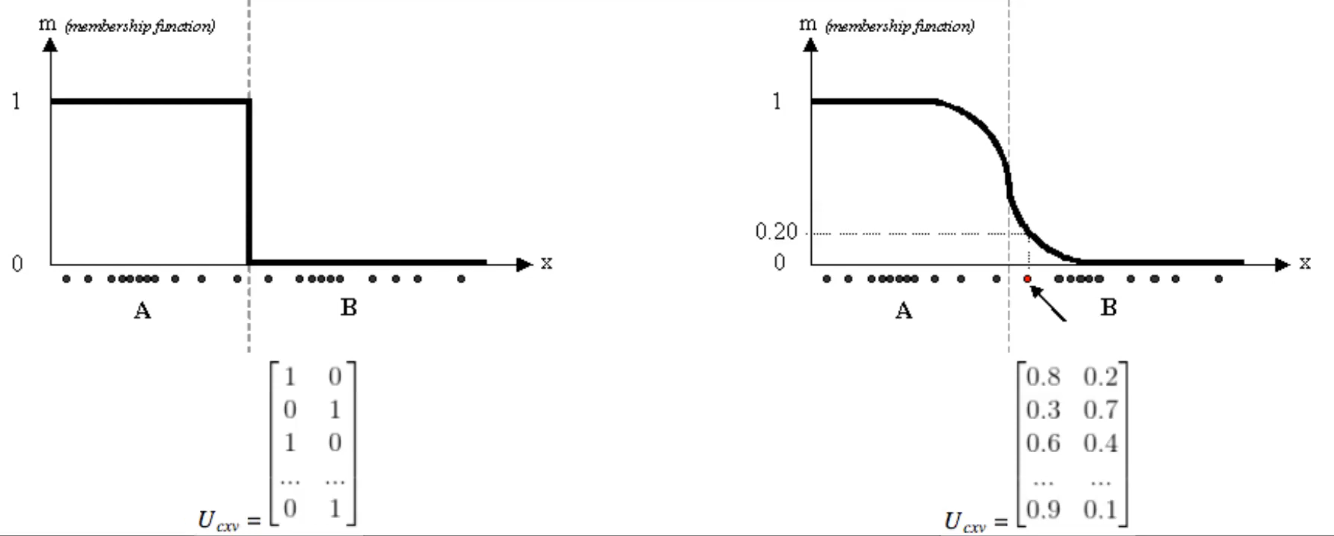
\includegraphics[height=6cm, width=12cm]{fuzzy_vs_kmeans}
\end{frame}

\begin{frame}{\lr{Fuzzy c-means}}
	\begin{center}
	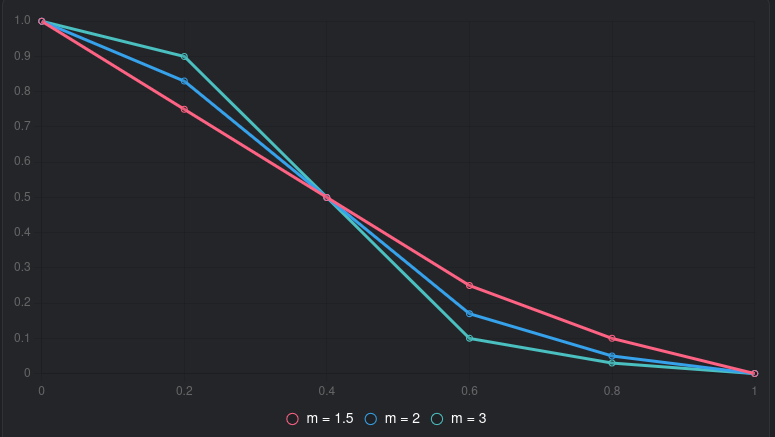
\includegraphics[height=4cm, width=8cm]{fuzzifier_1}\\
	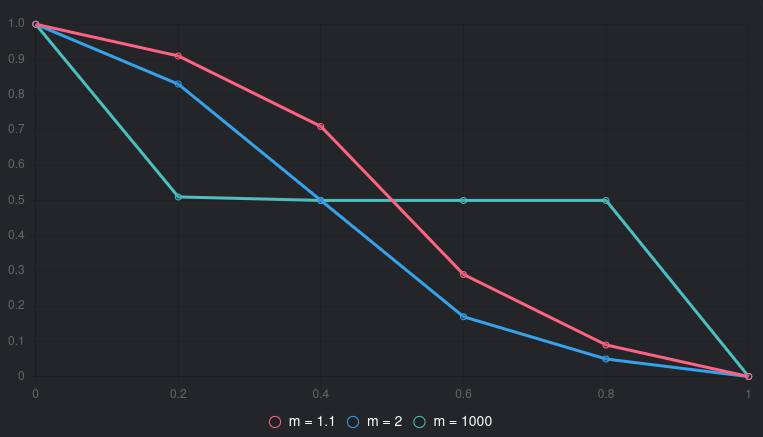
\includegraphics[height=4cm, width=8cm]{fuzzifier_2}
	\end{center}
\end{frame}

\begin{frame}{\lr{Appilcation of Fuzzy c-means}}
\begin{footnotesize}
این الگوریتم به دلیل انعطاف پذیری در خوشه بندی نرم، در حوزه های مختلفی کاربرد دارد:
\begin{enumerate}
	\item
پردازش تصویر 
	\begin{itemize}
		\item تقسیم بندی تصاویر مثل جداسازی بافت ها در تصاویر پزشکی \lr{MRI}
		\item کاهش نویز یا فشردگی تصاویر
	\end{itemize}
	\item 
تحلیل داده های زیستی 
	\begin{itemize}
		\item خوشه بندی ژن ها یا پروتئین ها بر اساس الگو.
		\item تشخیص الگو های بیماری در داده های پزشکی
	\end{itemize}
	\item بازاریابی و تحلیل داده 
	\begin{itemize}
		\item گروه بندی مشتریان بر اساس رفتار خرید با درجات عضویت مختلف 
		\item تحلیل داده های شبکه اجتماعی برای شناسایی جوامع
	\end{itemize}
\item هوش مصنوعی و یادگیری ماشین 
\begin{itemize}
	\item پیش پردازش داده ها برای بهبود عملکرد مدل های یادگیری ماشین 
	\item ترکیب با الگوریتم های دیگر مثل شبکه های عصبی
\end{itemize}
\end{enumerate}

	
\end{footnotesize}
\end{frame}
\begin{frame}{پیاده سازی}
	
	\section{خوشه بندی تصاویر  با الگوریتم \lr{FCM}}
\begin{footnotesize}
\begin{enumerate}
	\item 
	خواندن تصاویر :
	
	تصویر خاکستری یا رنگی با استفاده از کتابخانه های \lr{OpenCV} یا \lr{PIL} خوانده می شود.
\[
	I(x,y) \; \rightarrow \; Intensity \; or \; RGB
\]
\begin{center}
\begin{scriptsize}
 $Grayscale:\; \; I \in \; R^{H \times W} \quad ,RGB:\; I \; \in \; R^{H \times W \times3}$ 
\end{scriptsize}
\end{center}

	\item 
	تبدیل به بردار ویژگی :
	
	هر پیکسل به یک بردار ویژگی تبدیل می شود.
	
تصویر با ابعاد $W \times H$ (ارتفاع و عرض) به یک ماتریس $d \times N$ که $W \times H = N$ تعداد پیکسل ها و \lr{d} تعداد ویژگی هاست.
\[X=
 \begin{bmatrix}
	x_1\\
	x_2\\
	\vdots\\
	x_N\\
\end{bmatrix}
, \quad x_i \in \; R^d \]

\[x_i \; = \; [R,G,B,x,y]\]
\end{enumerate}
\end{footnotesize}
\end{frame}

\begin{frame}{پیاده سازی}
	\begin{footnotesize}
		\begin{enumerate}
			\item[3.]
	نرمال سازی داده ها:

مقادیر ویژگی ها باید نرمال سازی شود (مثلا در بازه [0,1]) تا فاصله اقلیدسی در \lr{FCM} معنا دار شود.
\[
x^{\prime} \; = \; \frac{x-x_{\min}}{x_{\max} - x_{\min}}
\]

\begin{center}
	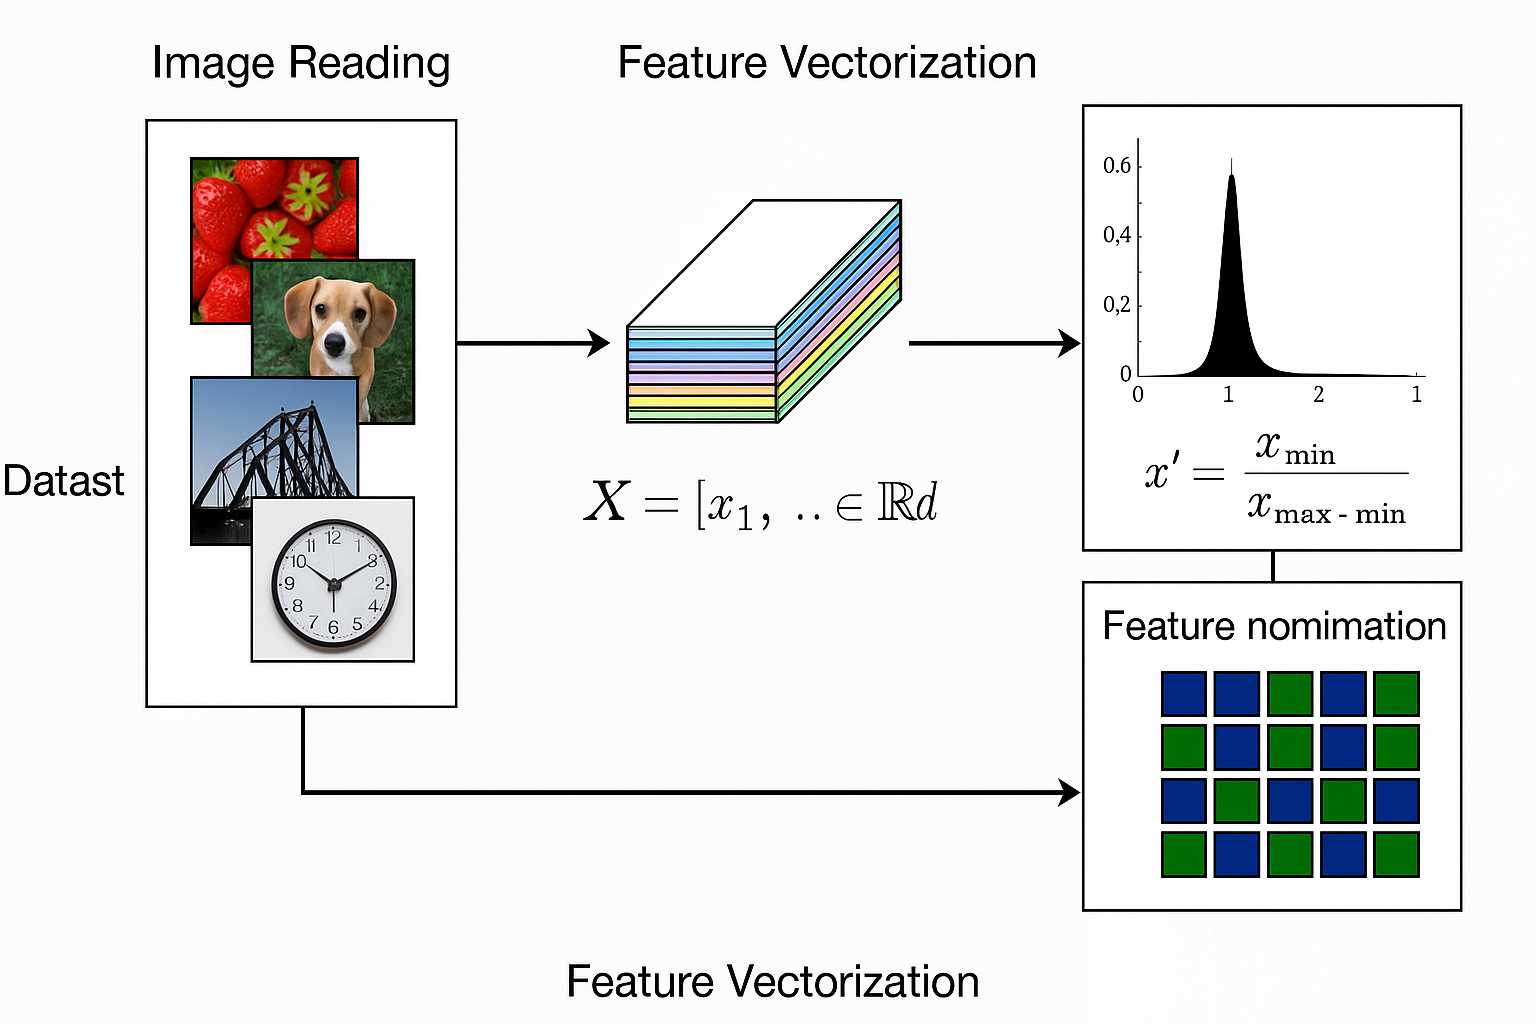
\includegraphics[height=6cm, width=10cm]{image_in_clustering}
\end{center}
		\end{enumerate}
	\end{footnotesize}

\end{frame}

\begin{frame}{معیار های ارزیابی مدل}
\section{ معیار های ارزیابی خوشه بندی }
\begin{itemize}
	\item \textbf{\lr{Silhoutte Score}}\\
میانگین تفاوت بین فاصله درون‌خوشه‌ای و فاصله به نزدیک‌ترین خوشه دیگر برای هر نمونه را اندازه‌گیری می‌کند. مقدار آن بین -1 تا 1 است؛ عدد بالاتر نشان‌دهنده‌ی تفکیک بهتر خوشه‌هاست.
	\item \textbf{\lr{Devies-Bouldin Index}}\\
نسبت میانگین پراکندگی در خوشه‌ها به فاصله بین خوشه‌ها را محاسبه می‌کند. مقدار کمتر نشان‌دهنده‌ی خوشه‌بندی بهتر است.
	\item \textbf{\lr{Calinski-Harabasz Index}}\\
نسبت بین پراکندگی بین‌خوشه‌ای به پراکندگی درون‌خوشه‌ای را می‌سنجد. مقدار بیشتر به معنای جداسازی و فشردگی بهتر خوشه‌هاست.
\end{itemize}	
\end{frame}

\begin{frame}{مقایسه خروجی ها}
	\begin{center}
		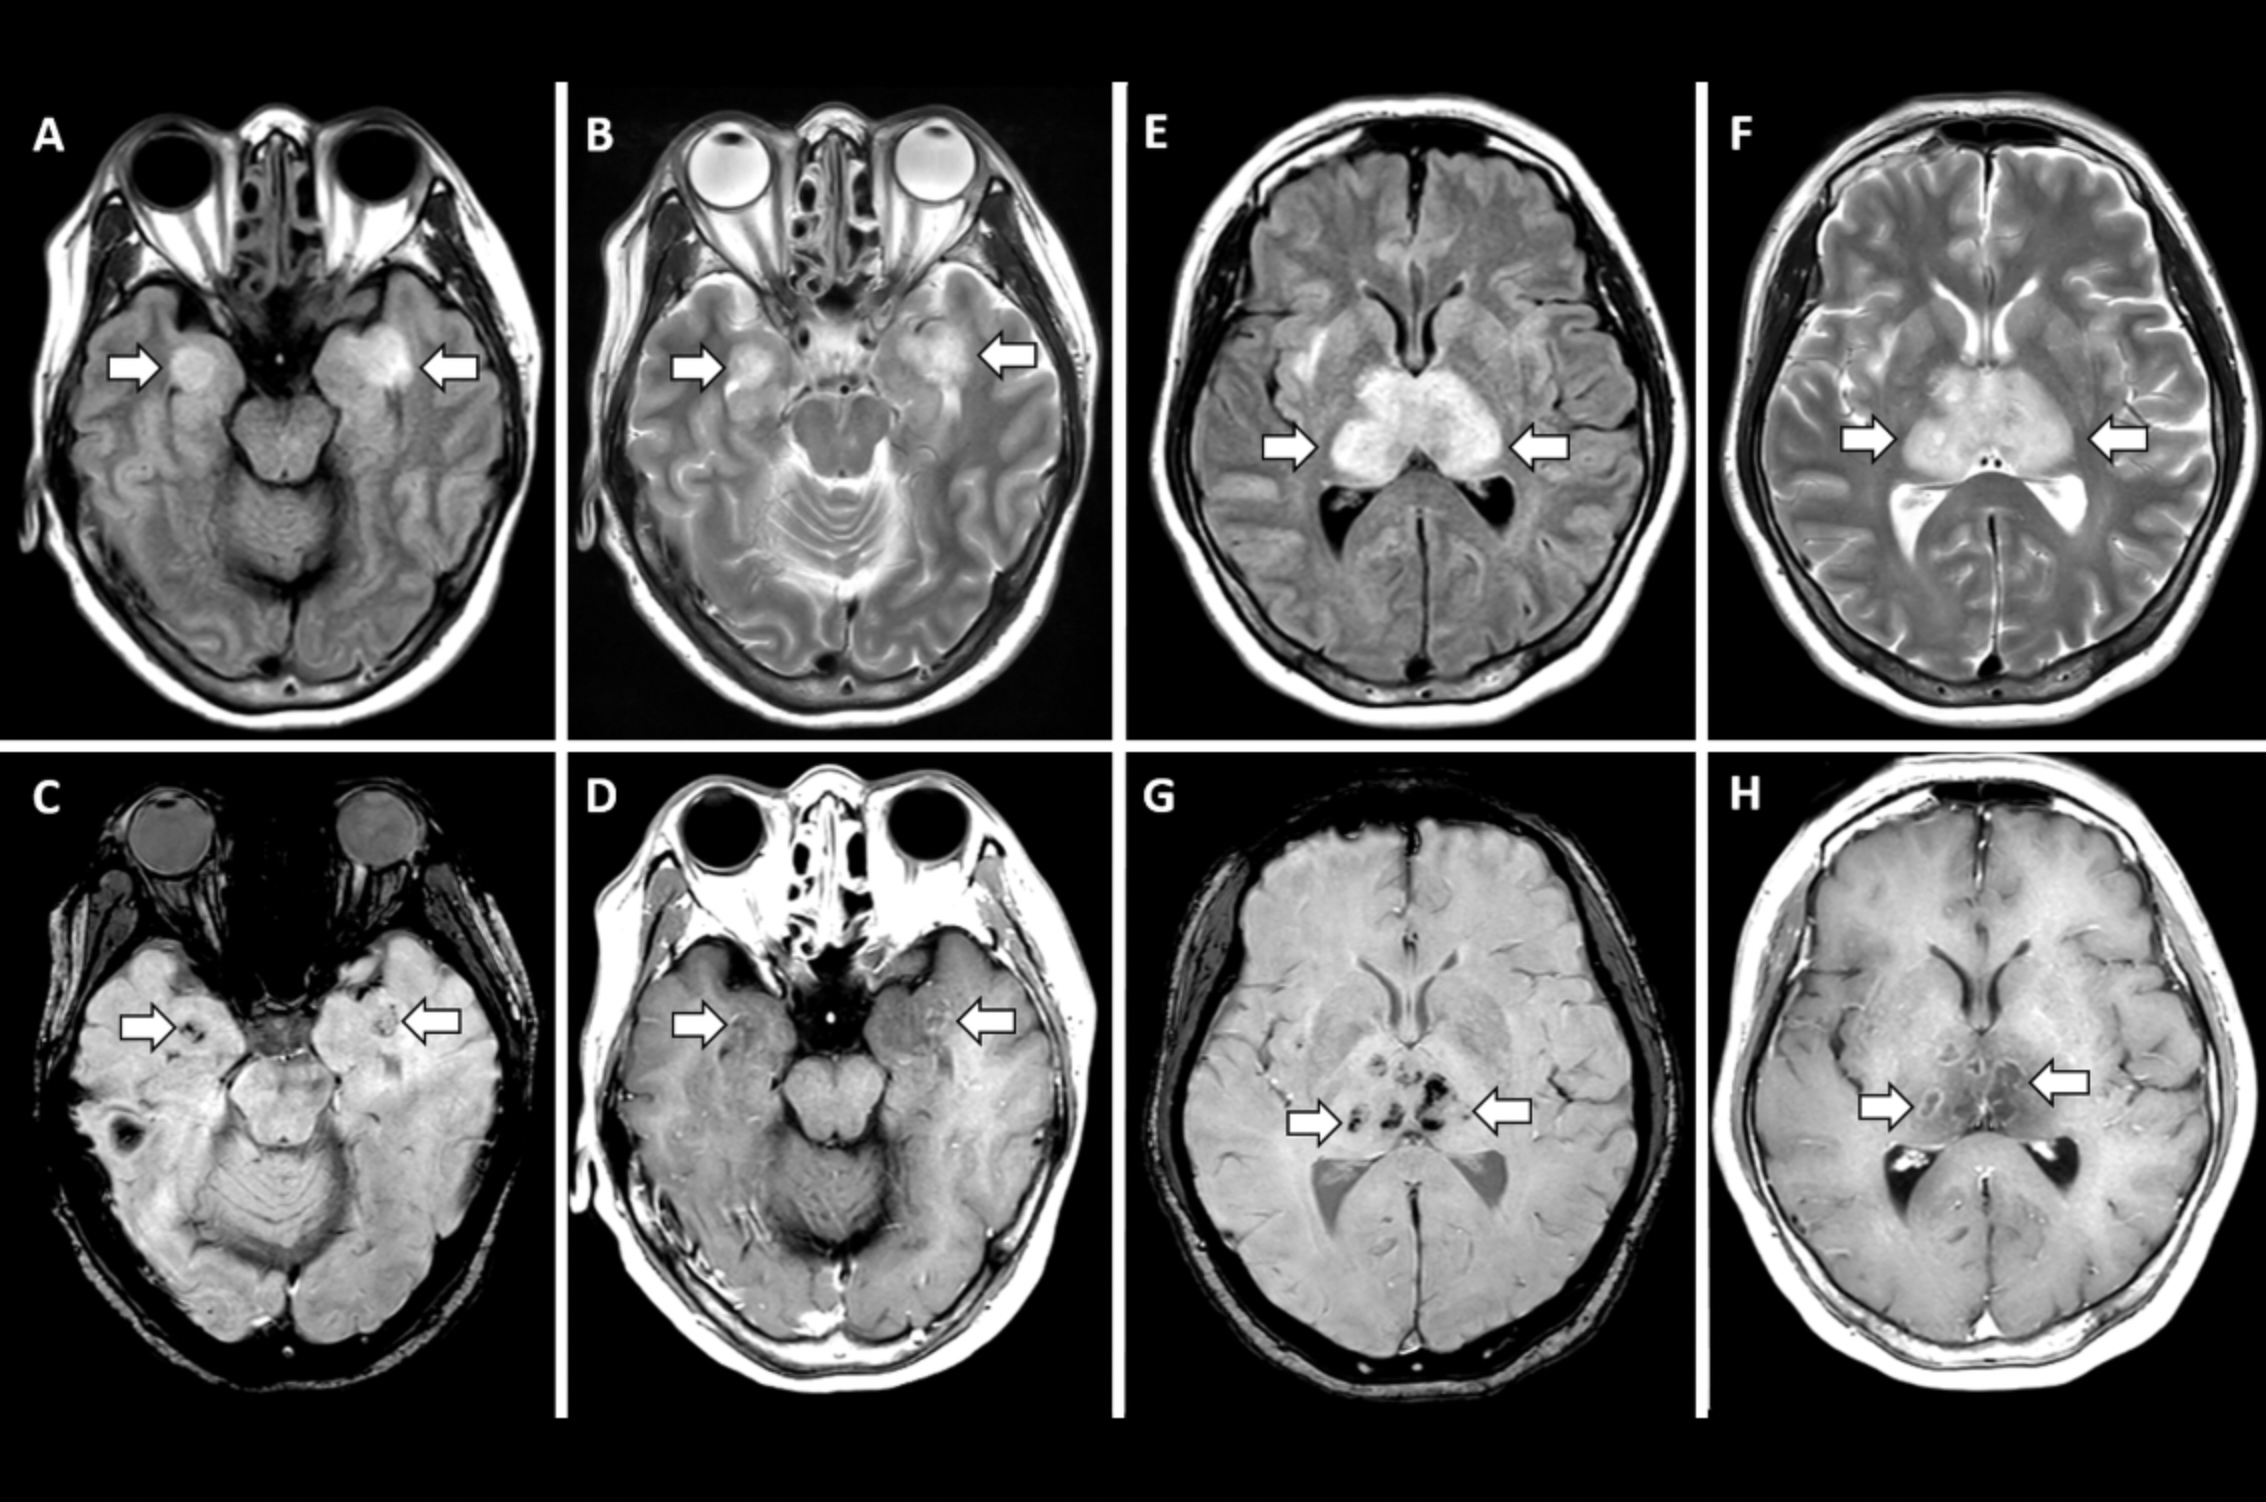
\includegraphics[height=5cm, width=10cm]{brain}
	\end{center}
\end{frame}
\begin{frame}{مقایسه خروجی ها}
	\begin{center}
		\begin{tabular}{c c}
 \lr{fuzzy c-means} & \lr{k-means}\\
		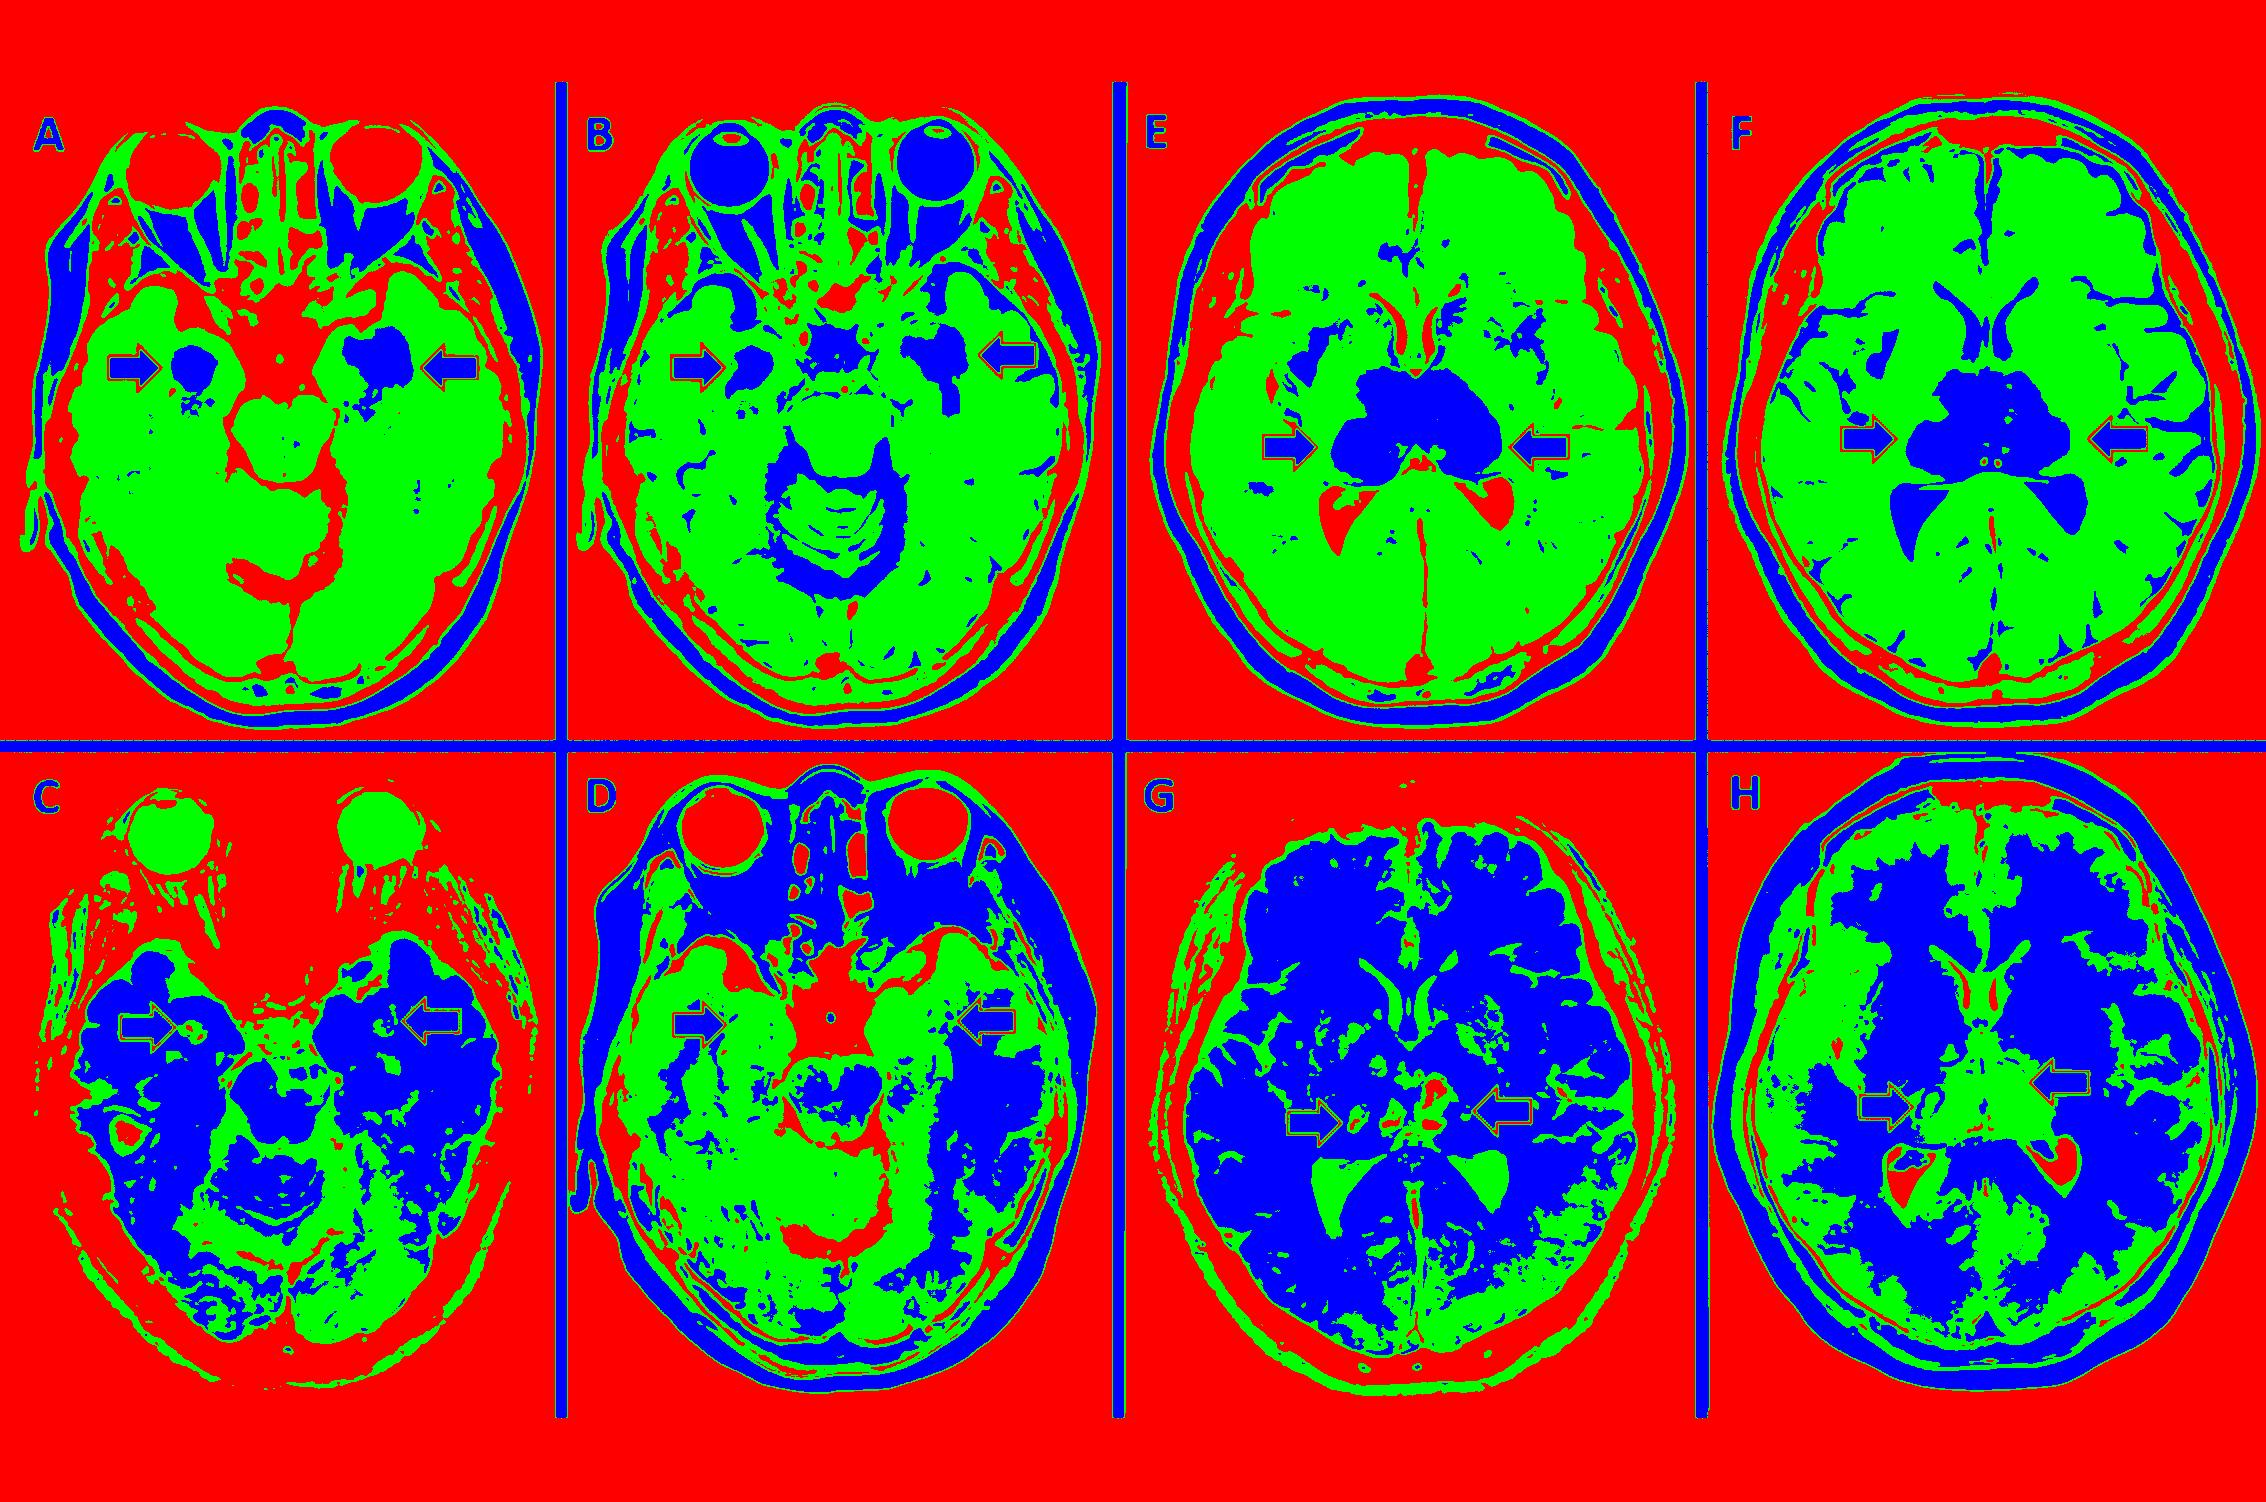
\includegraphics[height=4cm, width=5.5cm]{segmented_image}&
		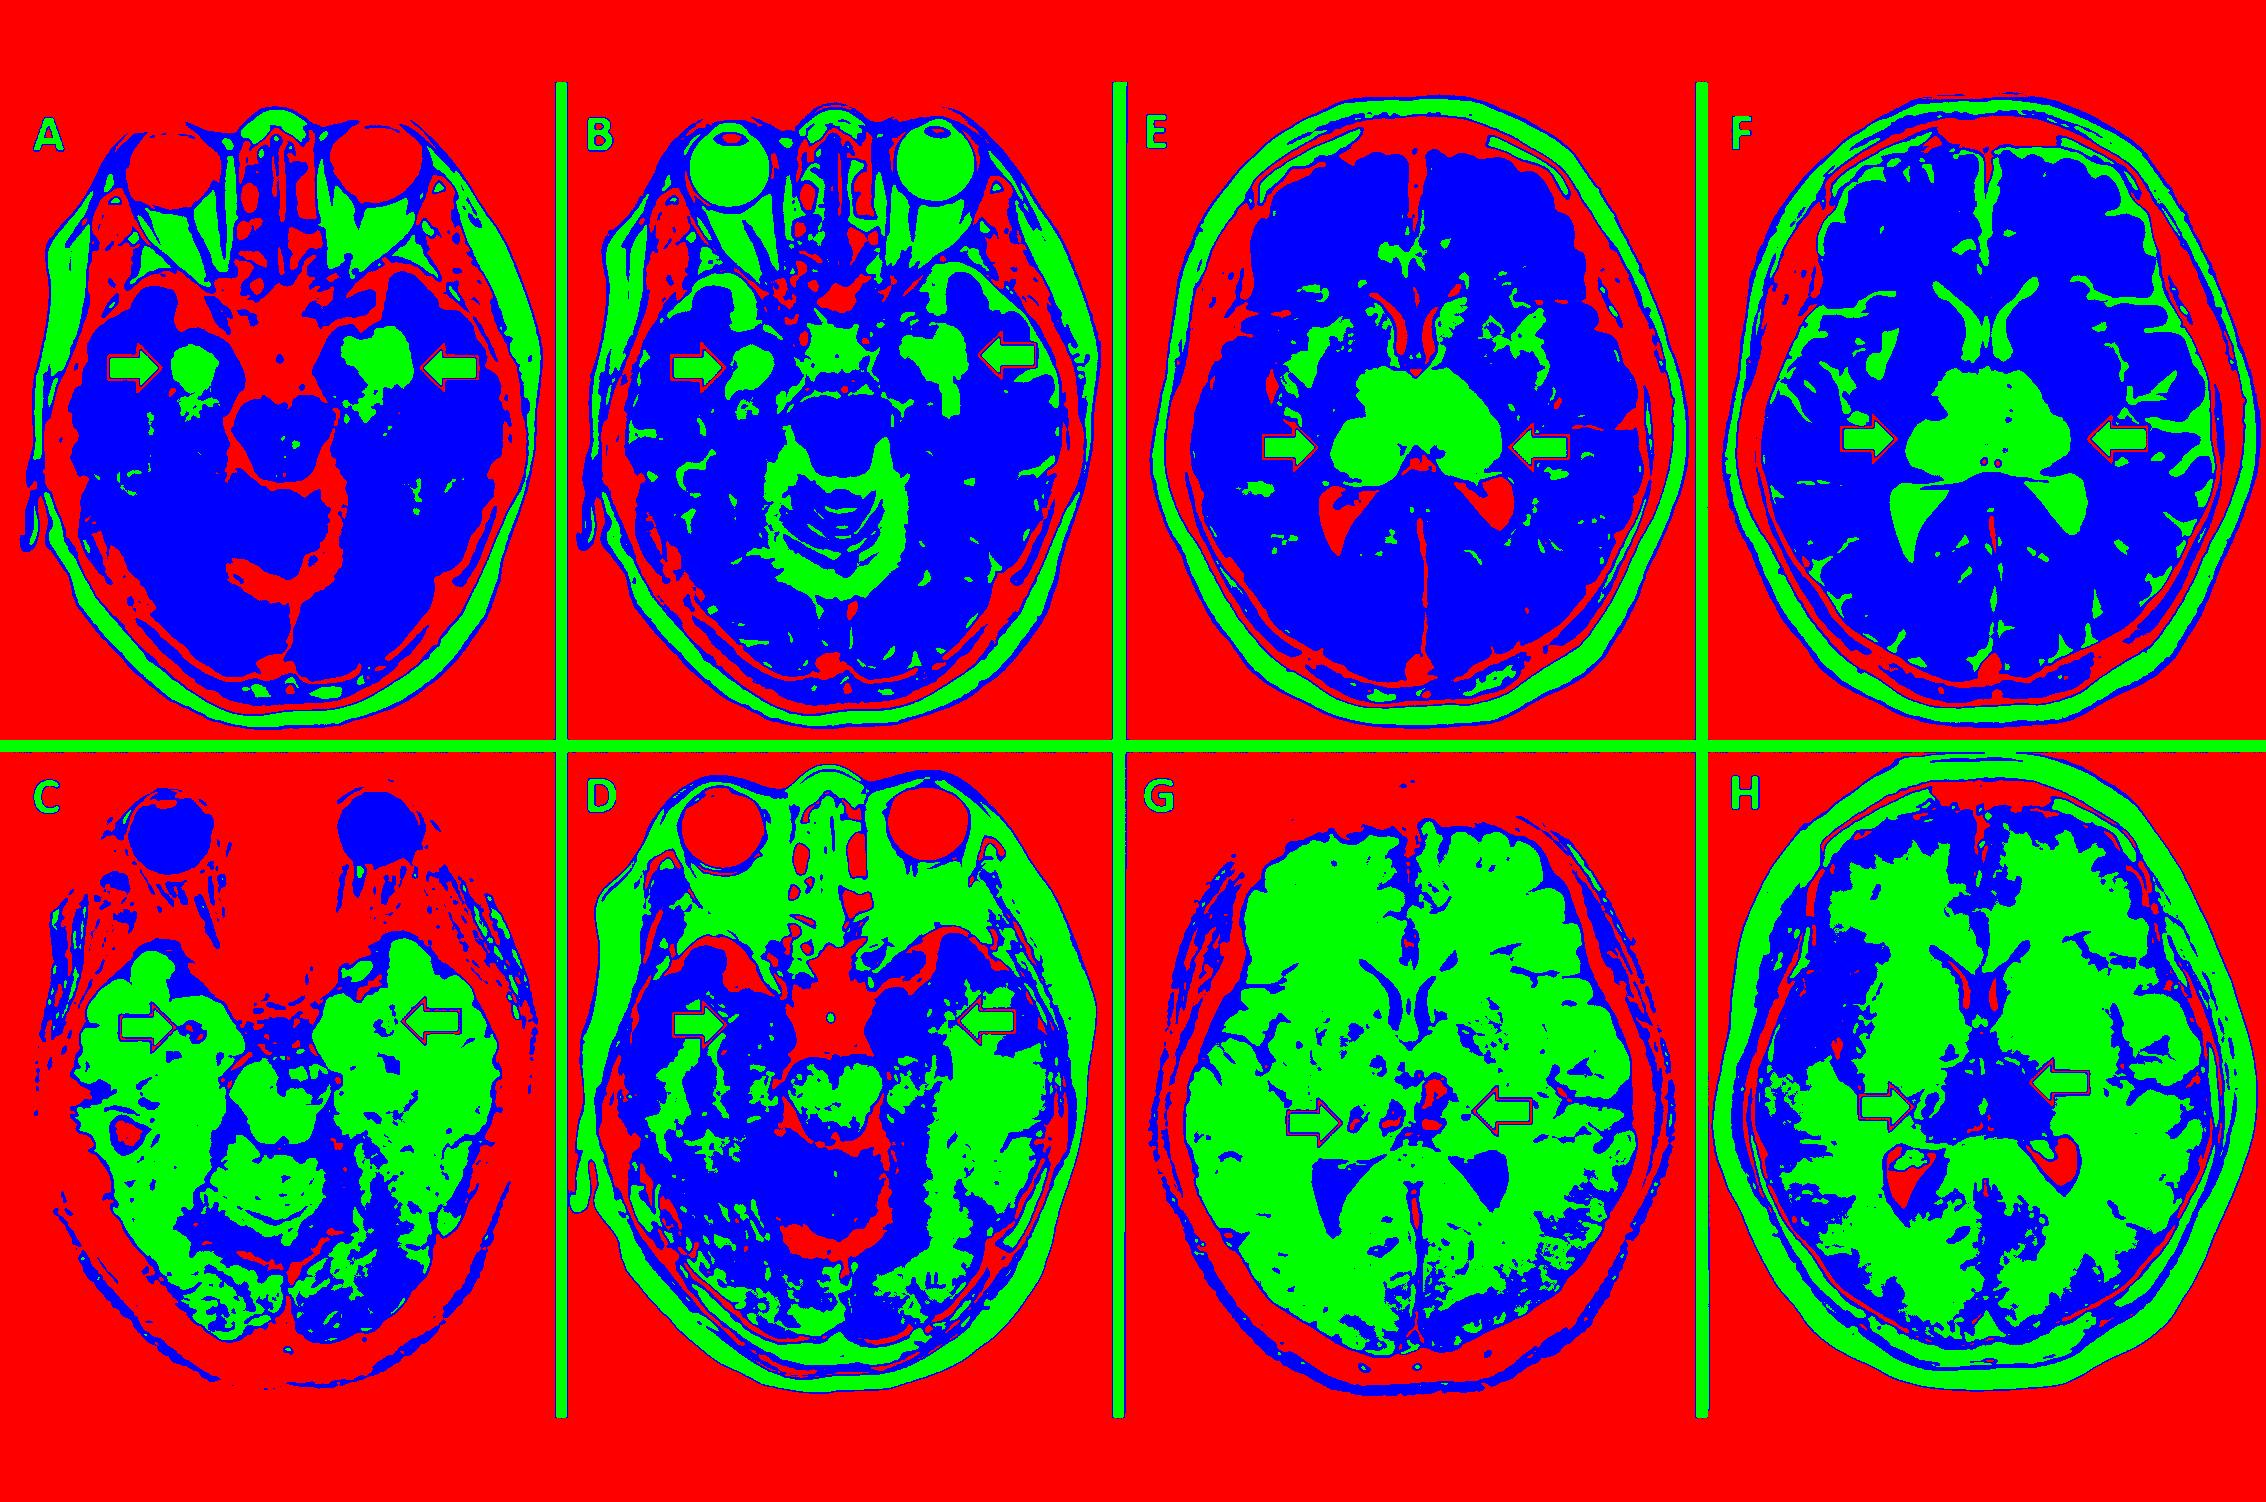
\includegraphics[height=4cm, width=5.5cm]{segmented_image_kmeans}\\
\end{tabular}
		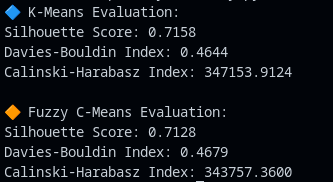
\includegraphics[height=2cm, width=3cm]{test1}
\end{center}
\end{frame}

\begin{frame}{مقایسه خروجی ها}
	\begin{center}
		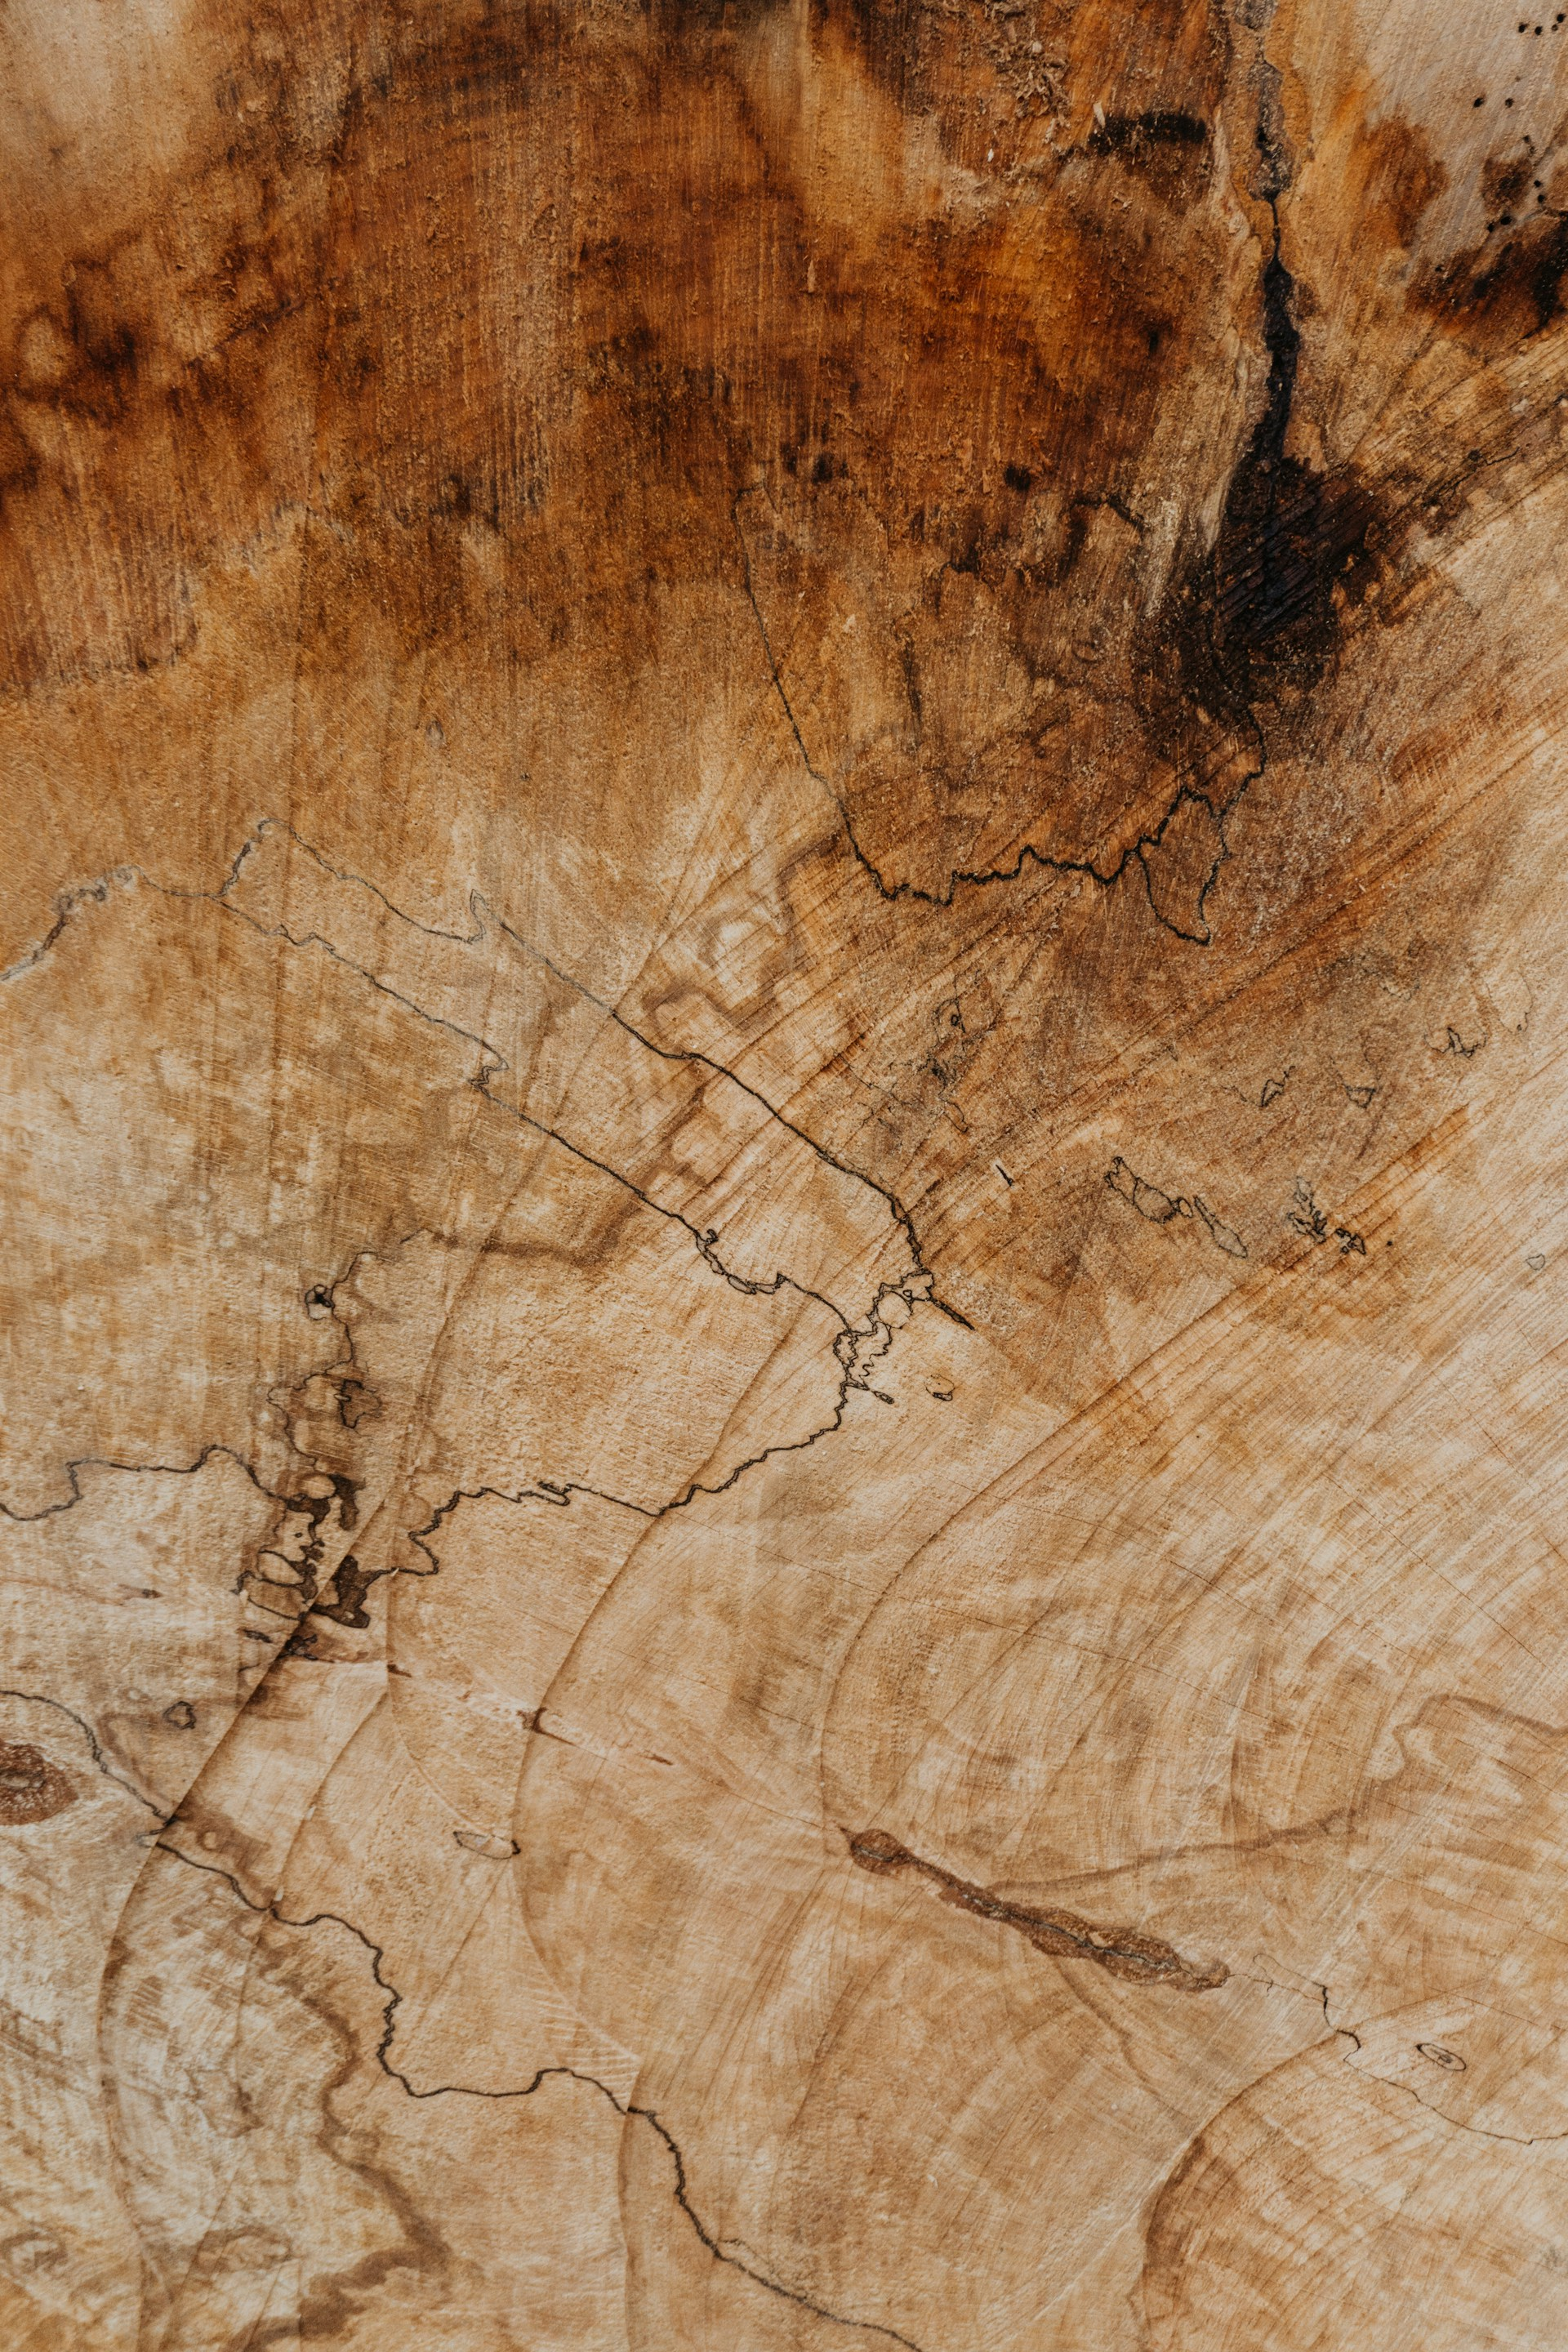
\includegraphics[height=5cm, width=10cm]{wood}
	\end{center}
\end{frame}
\begin{frame}{مقایسه خروجی ها}
	\begin{center}
		\begin{tabular}{c c}
			\lr{fuzzy c-means} & \lr{k-means}\\
			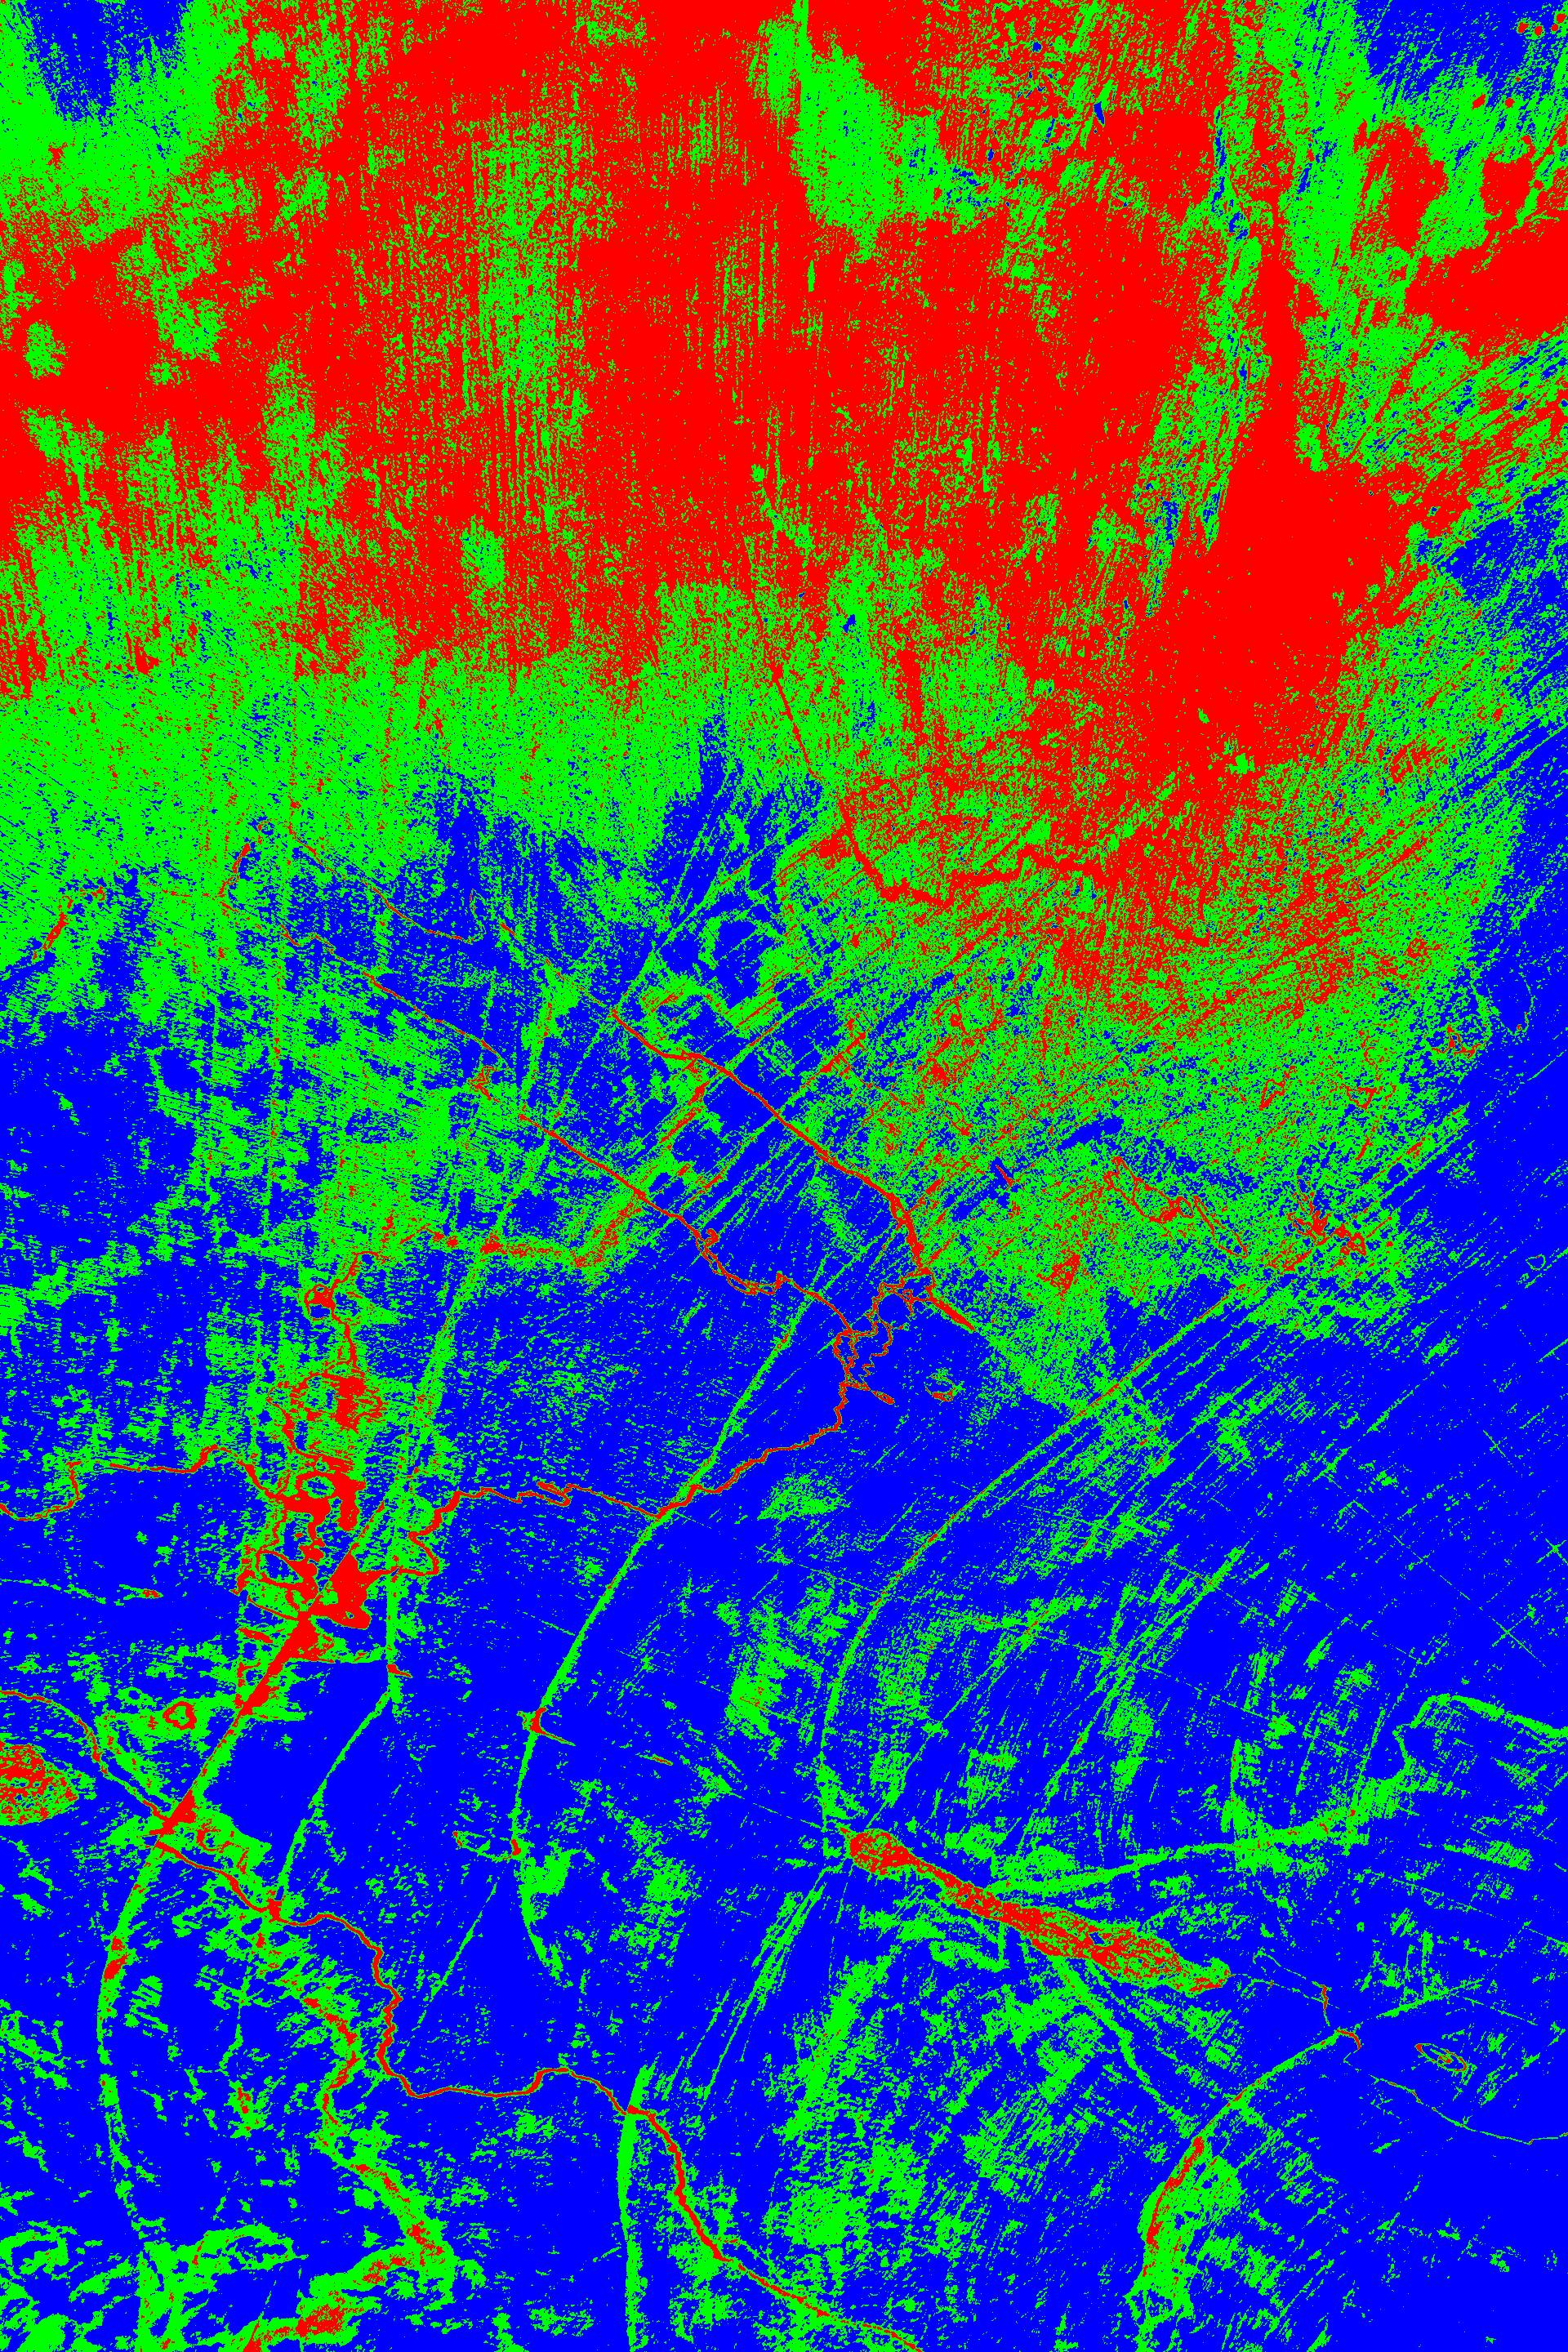
\includegraphics[height=4cm, width=5.5cm]{segmented_image2}&
			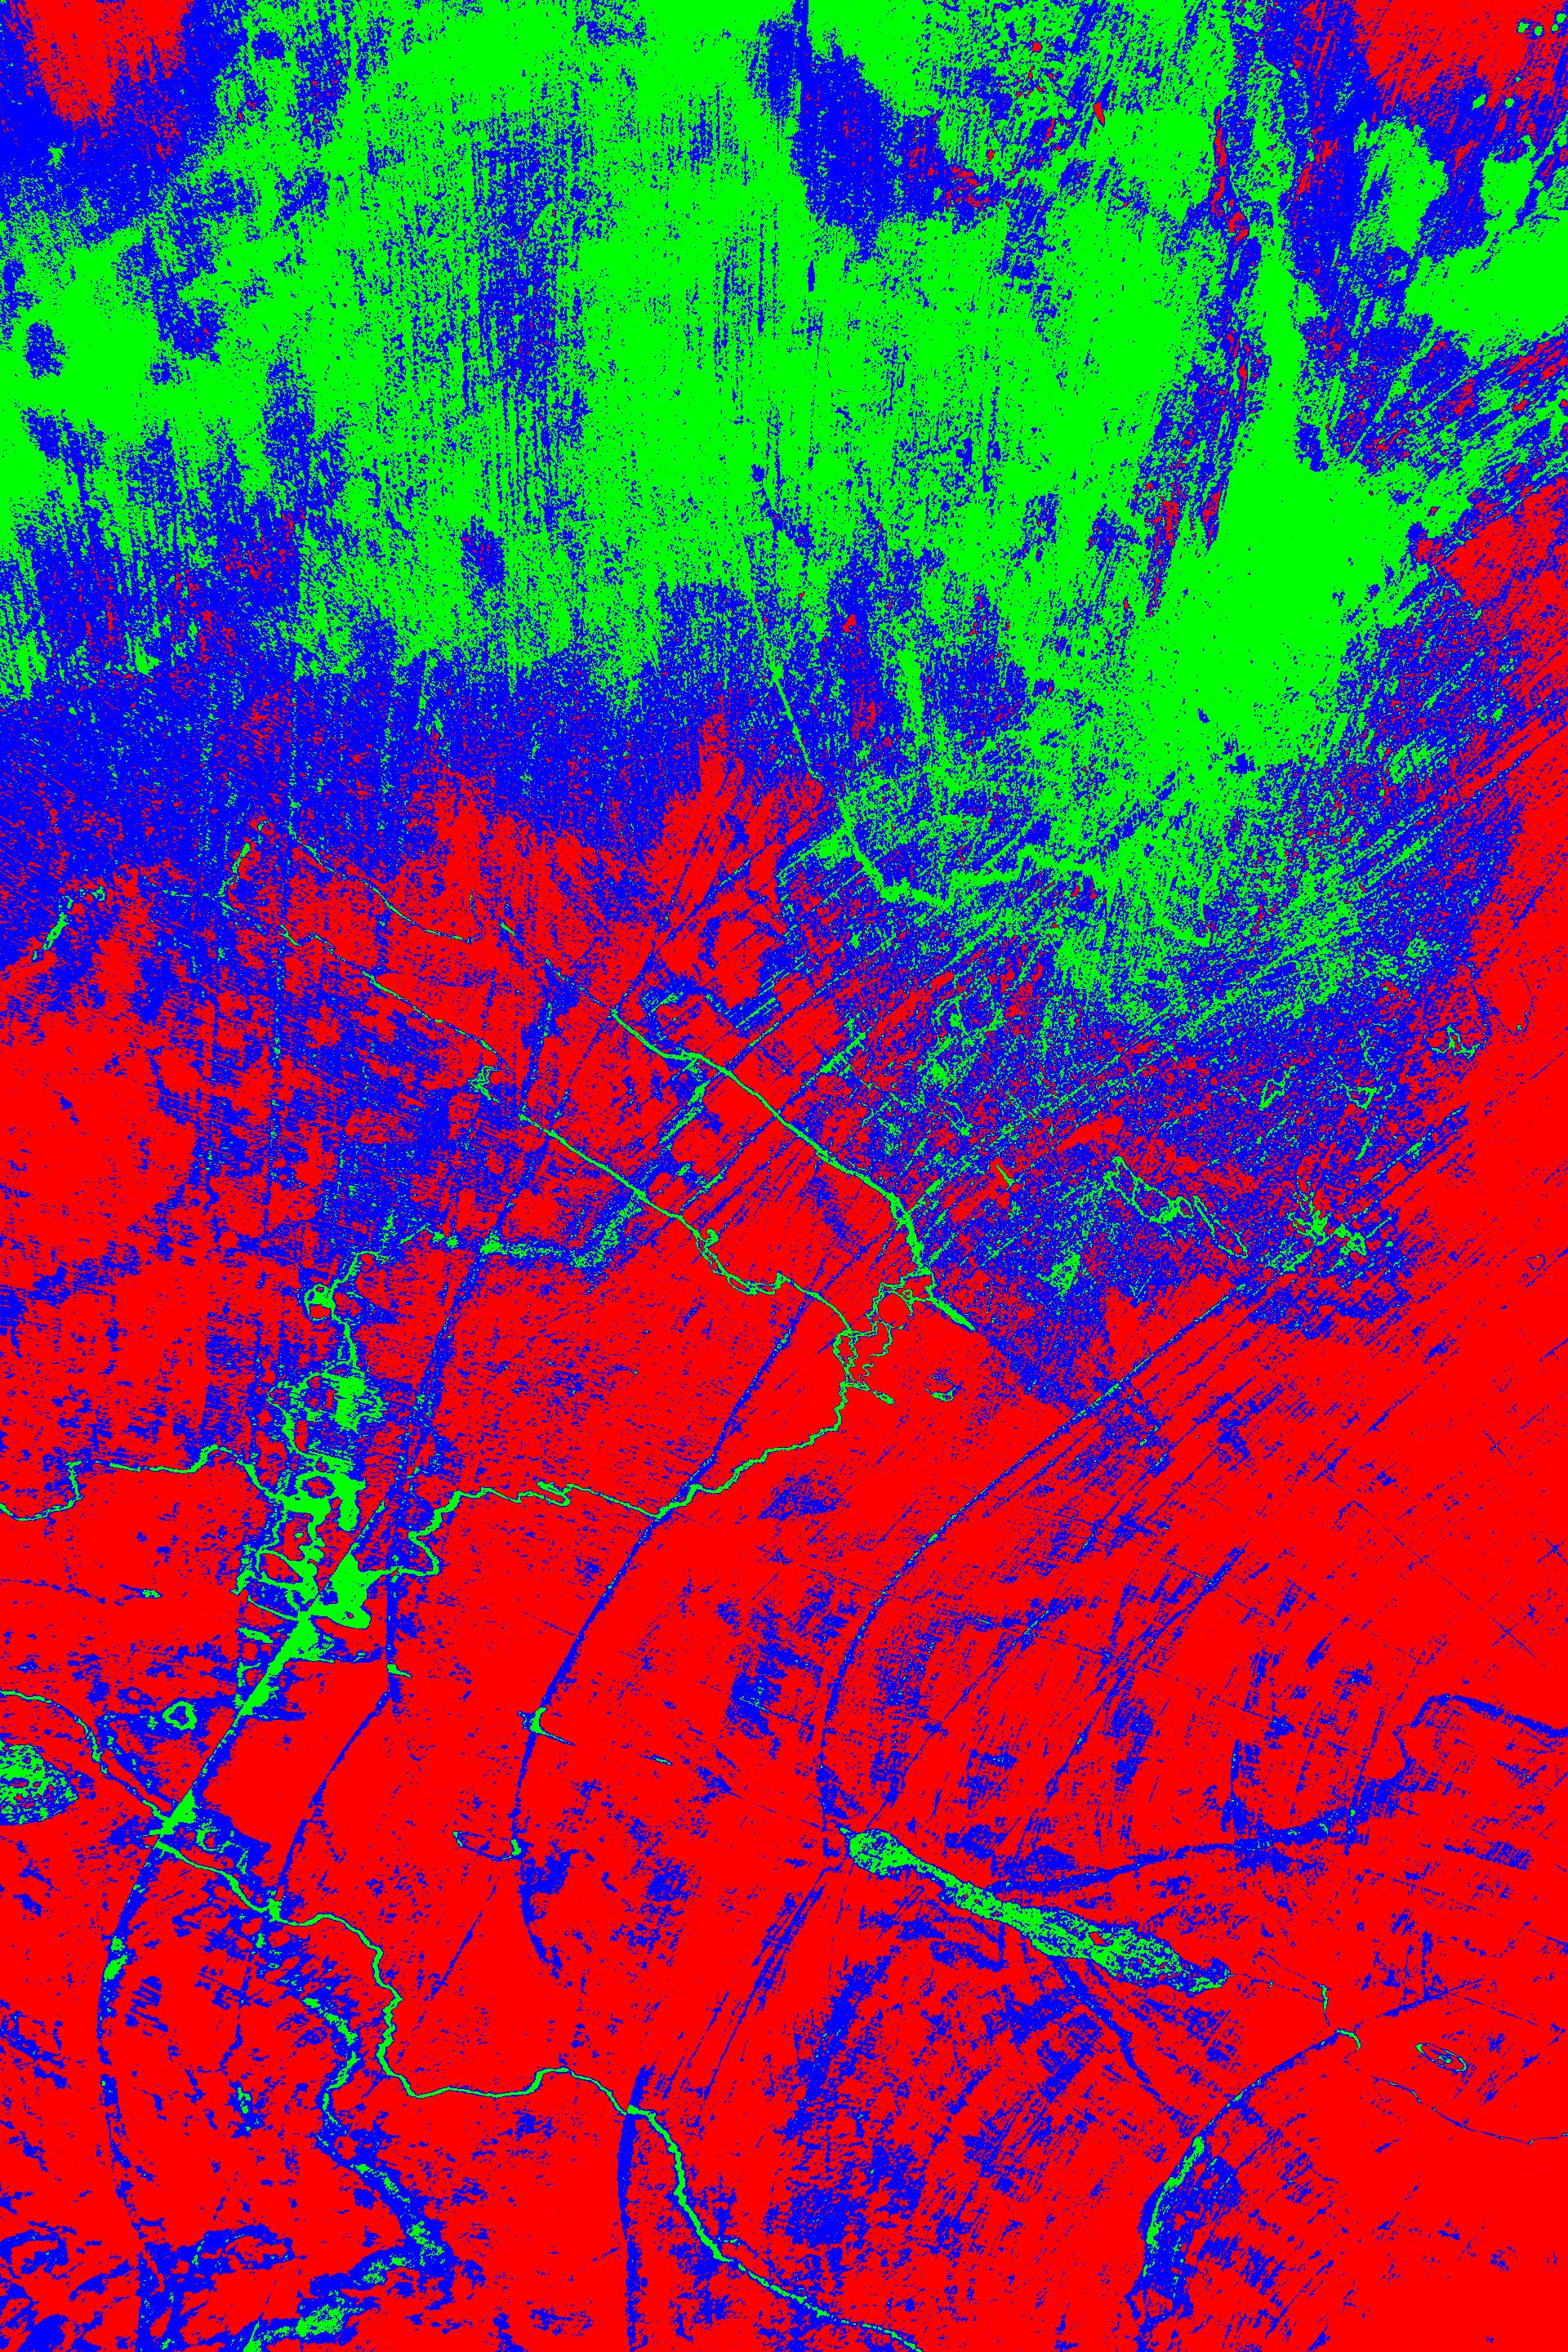
\includegraphics[height=4cm, width=5.5cm]{segmented_image_kmeans2}\\
		\end{tabular}
		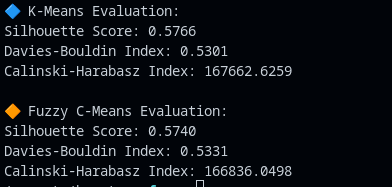
\includegraphics[height=2cm, width=3cm]{test2}
	\end{center}
\end{frame}

\begin{frame}{مقایسه خروجی ها}
	\begin{center}
		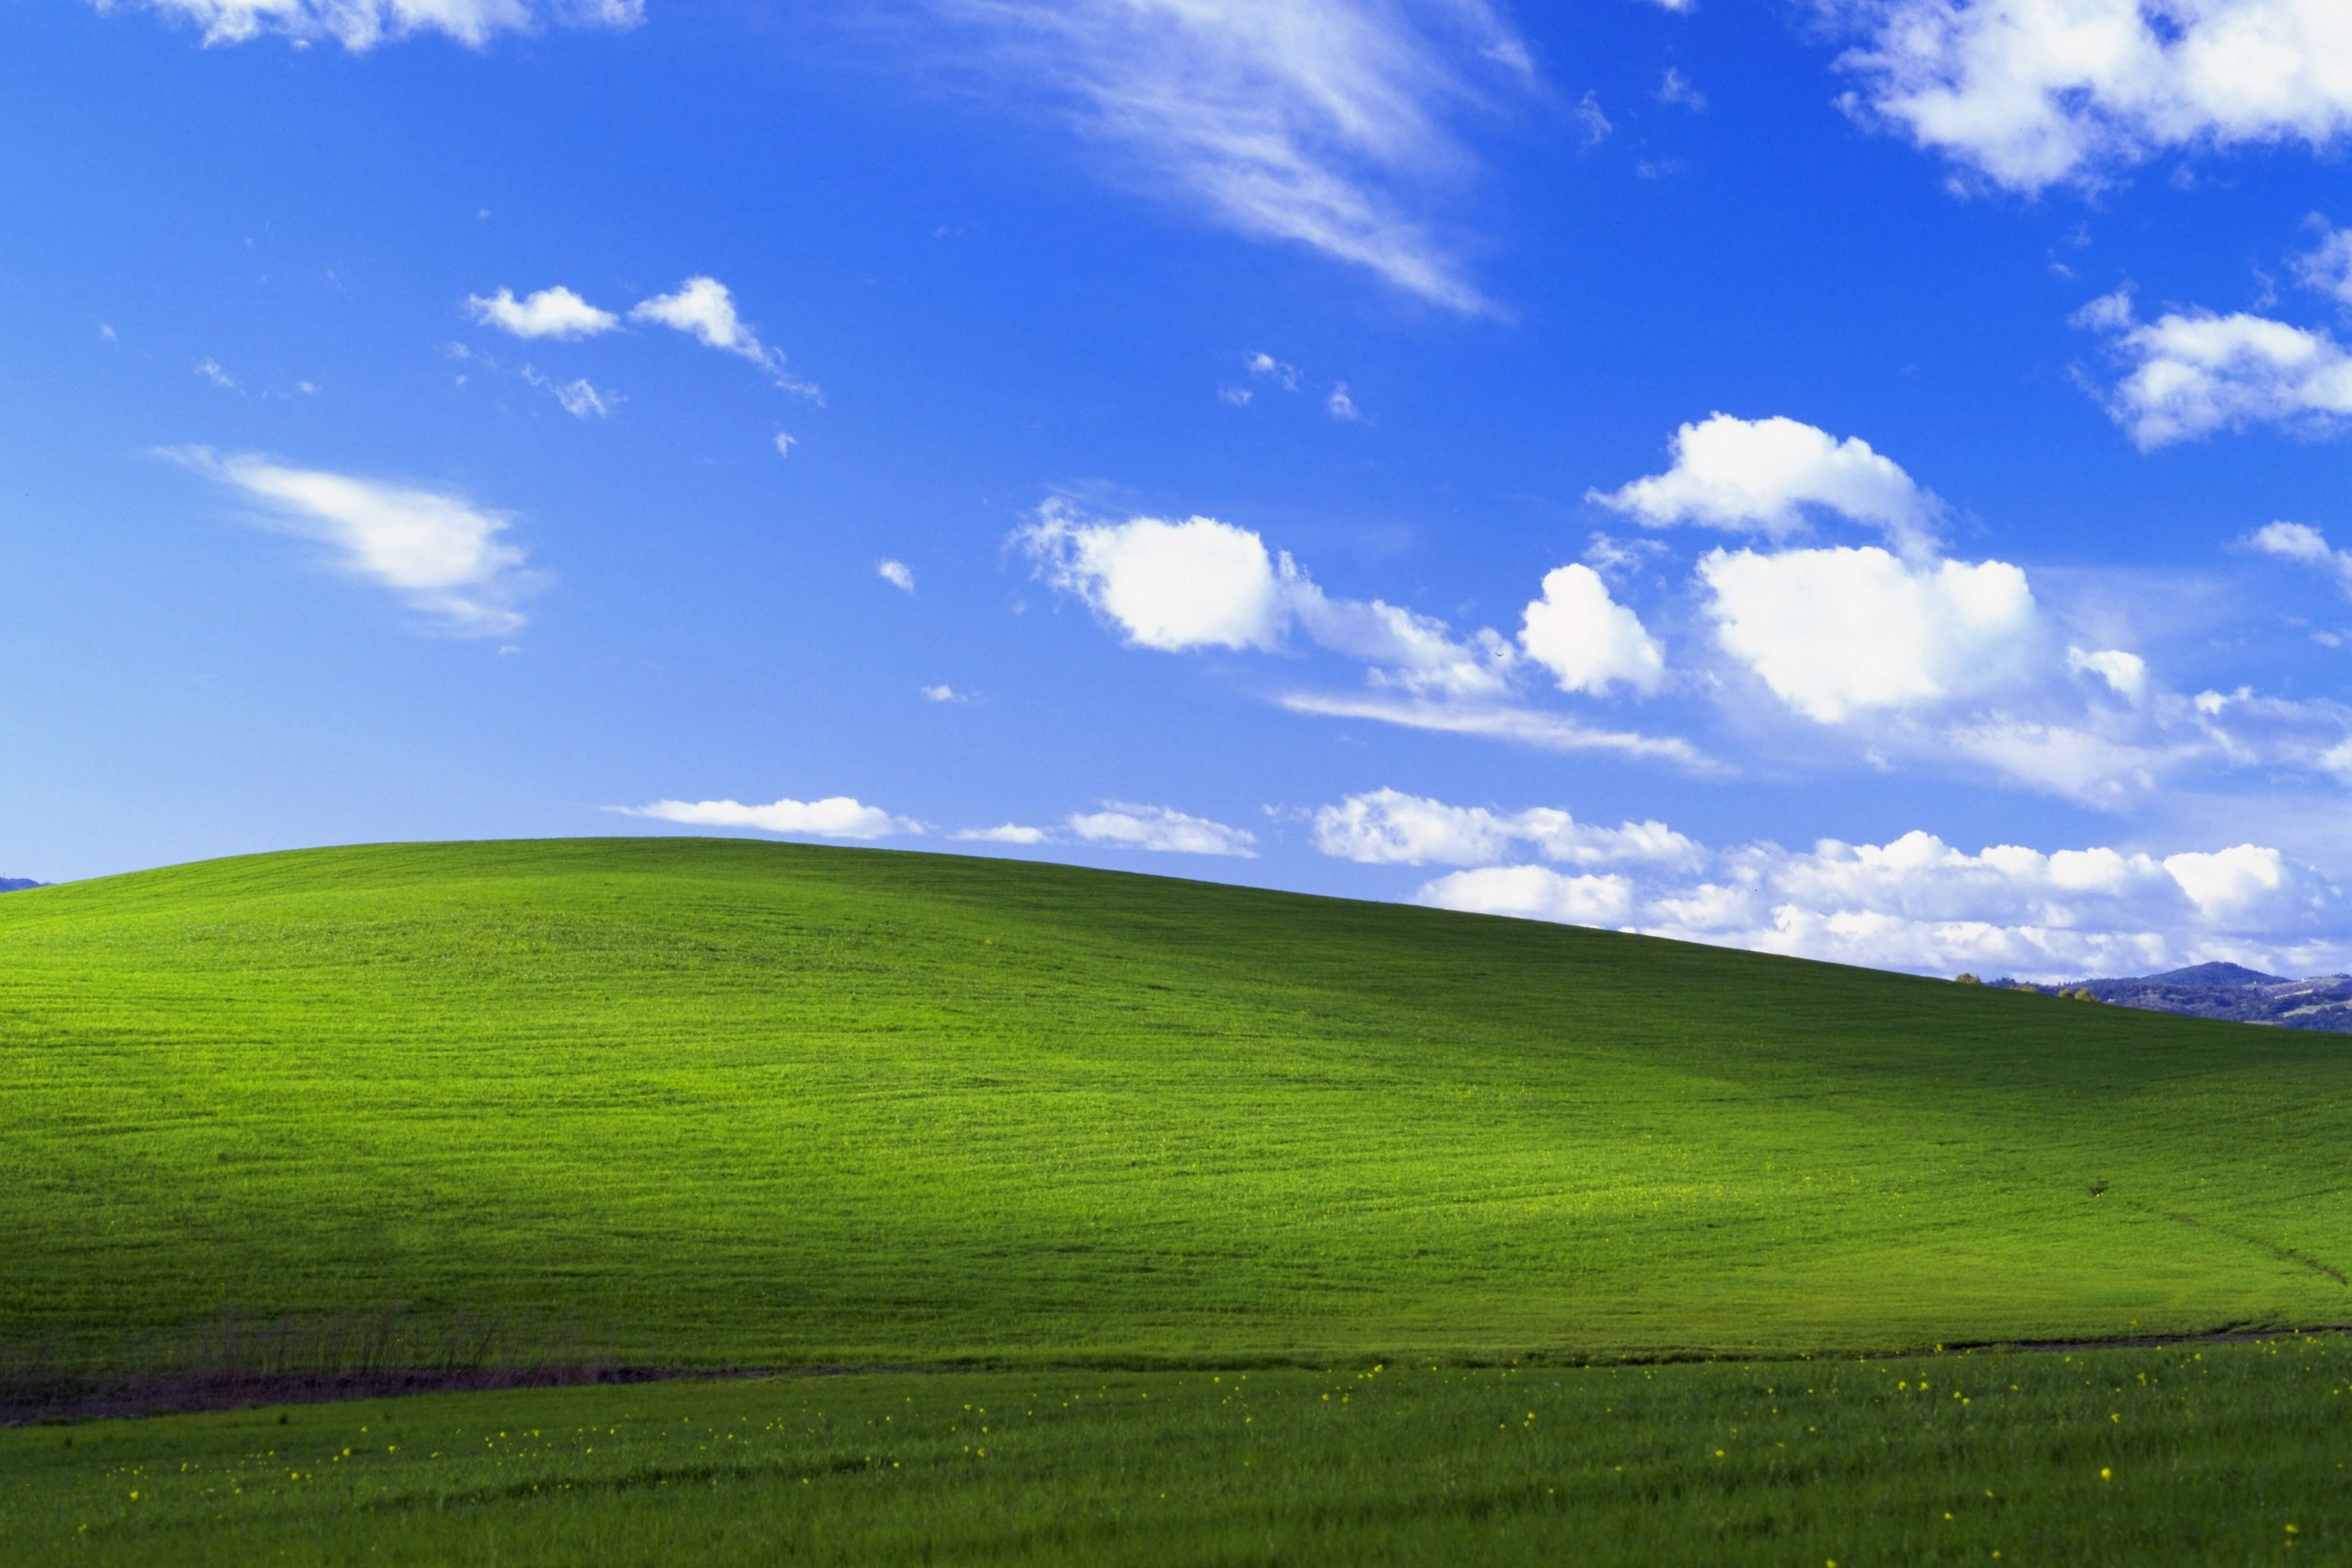
\includegraphics[height=5cm, width=10cm]{windowsXP}
	\end{center}
\end{frame}
\begin{frame}{مقایسه خروجی ها}
	\begin{center}
		\begin{tabular}{c c}
			\lr{fuzzy c-means} & \lr{k-means}\\
			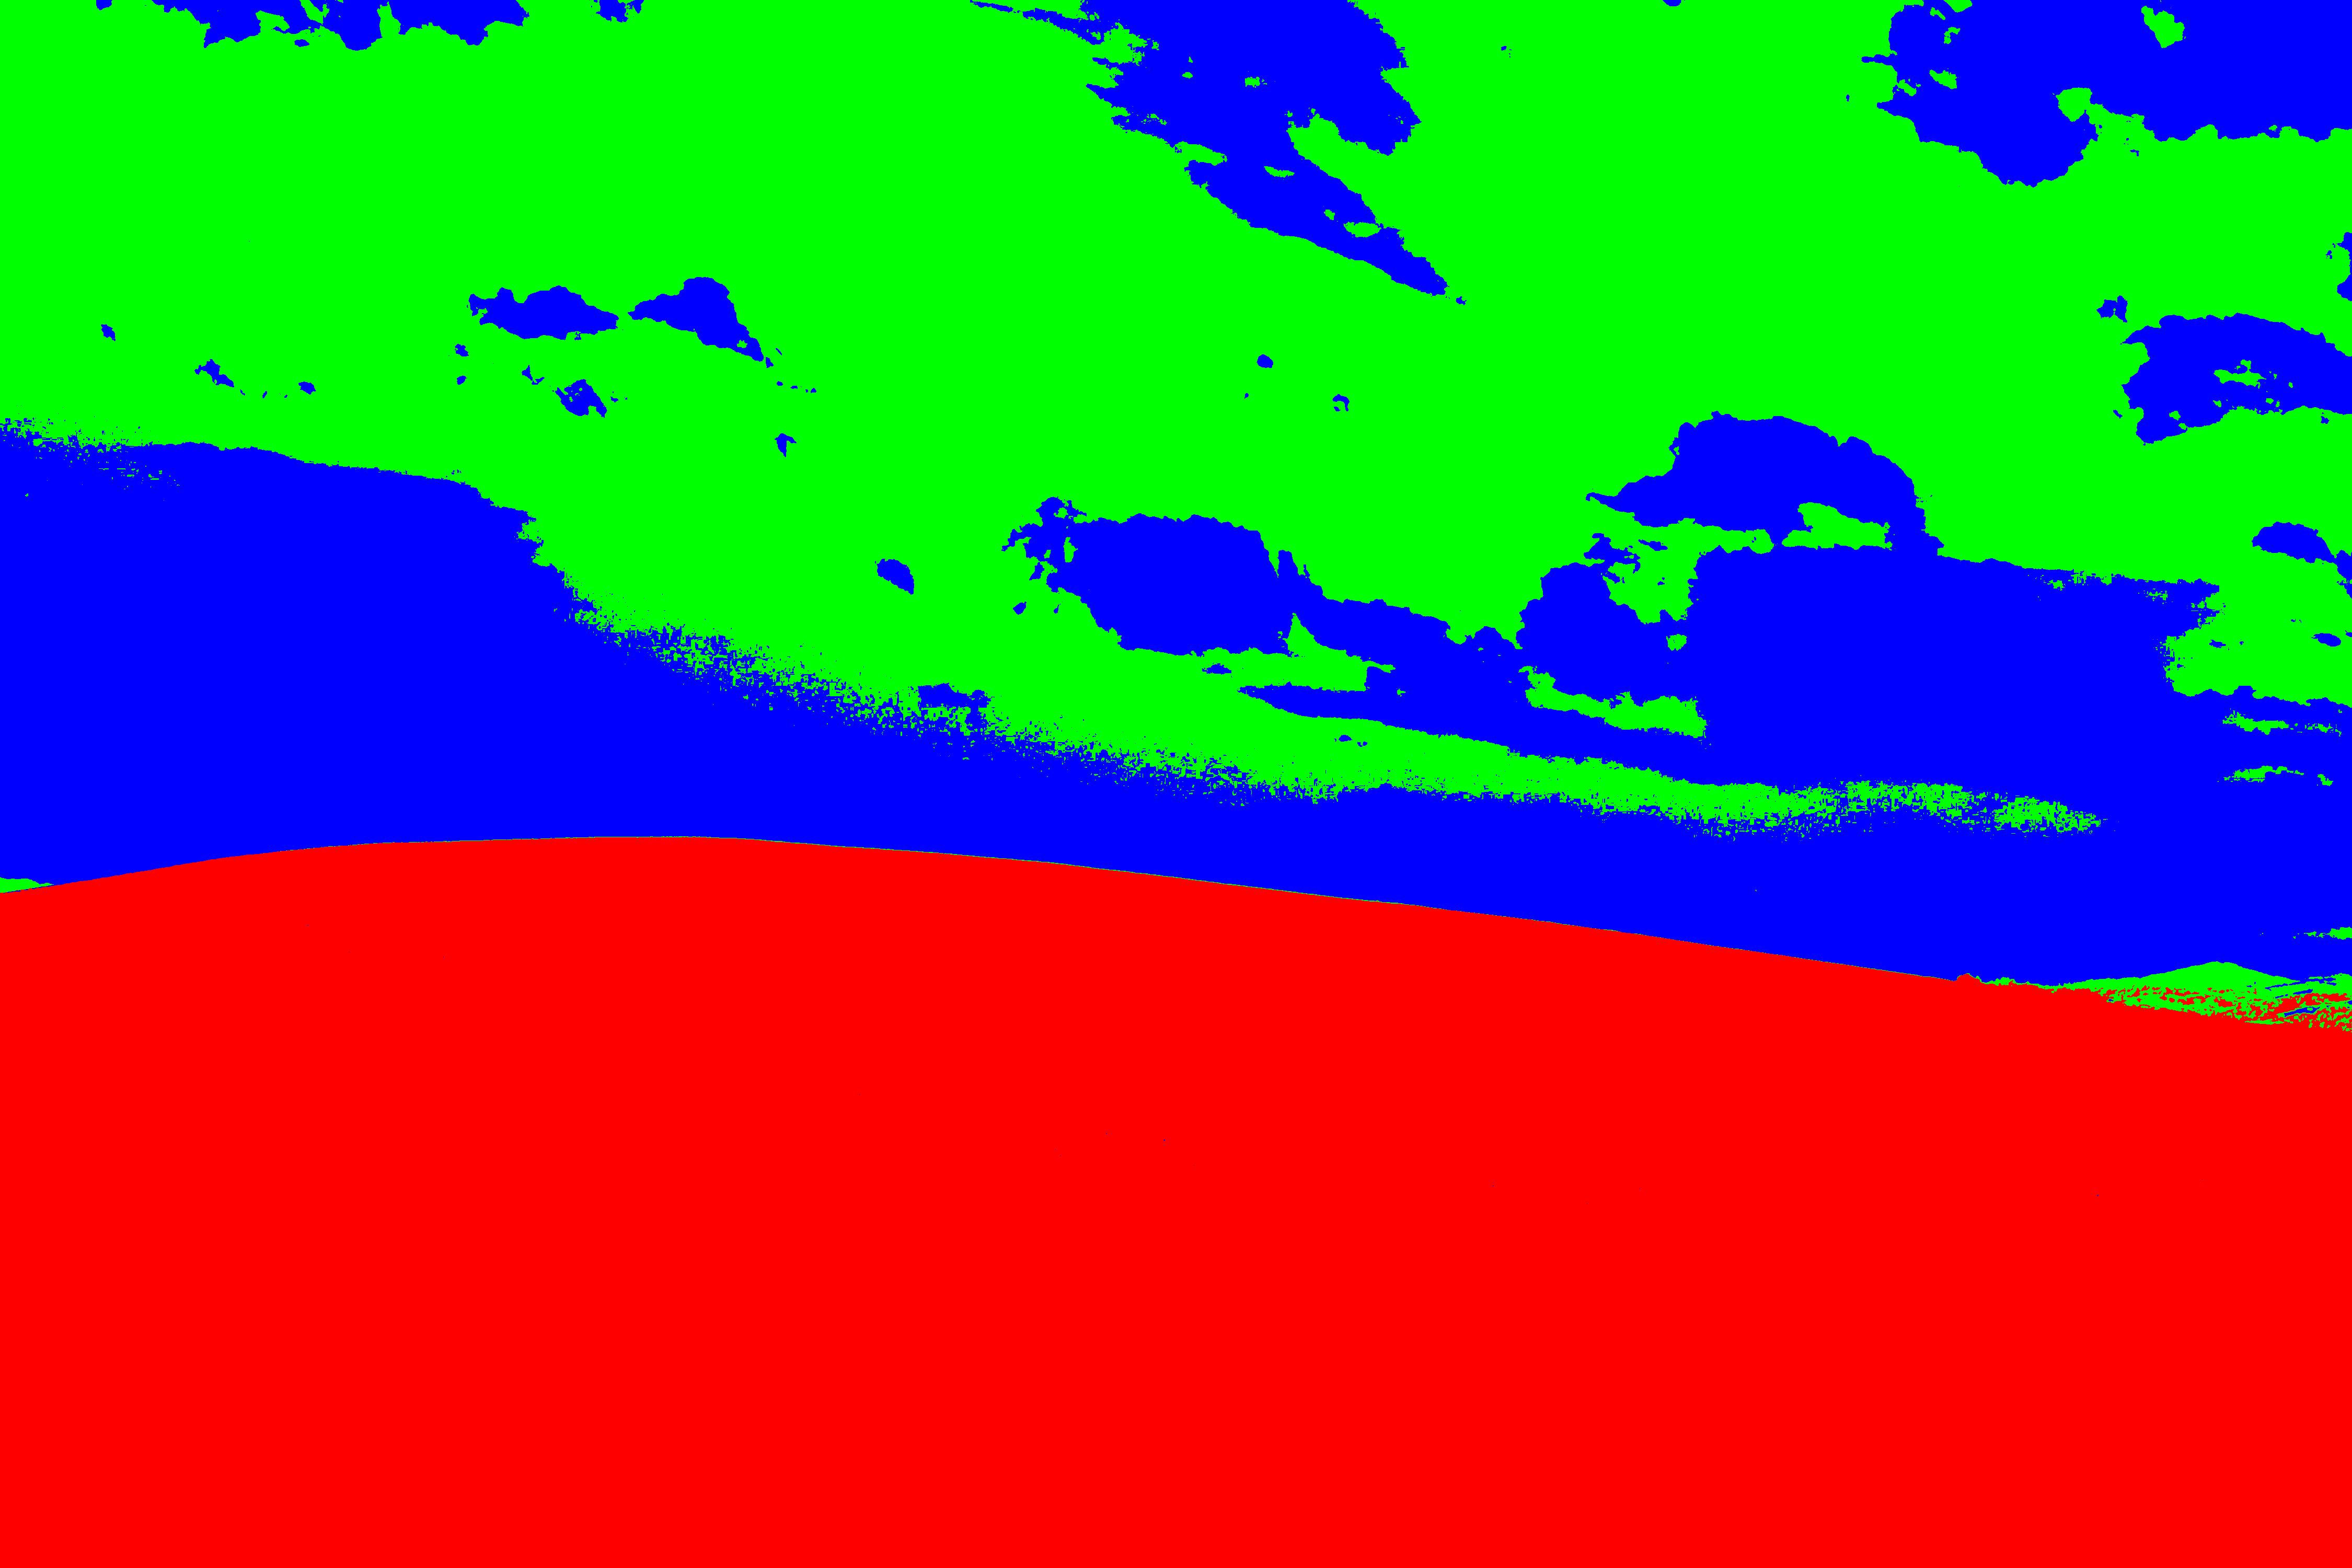
\includegraphics[height=4cm, width=5.5cm]{segmented_image1}&
			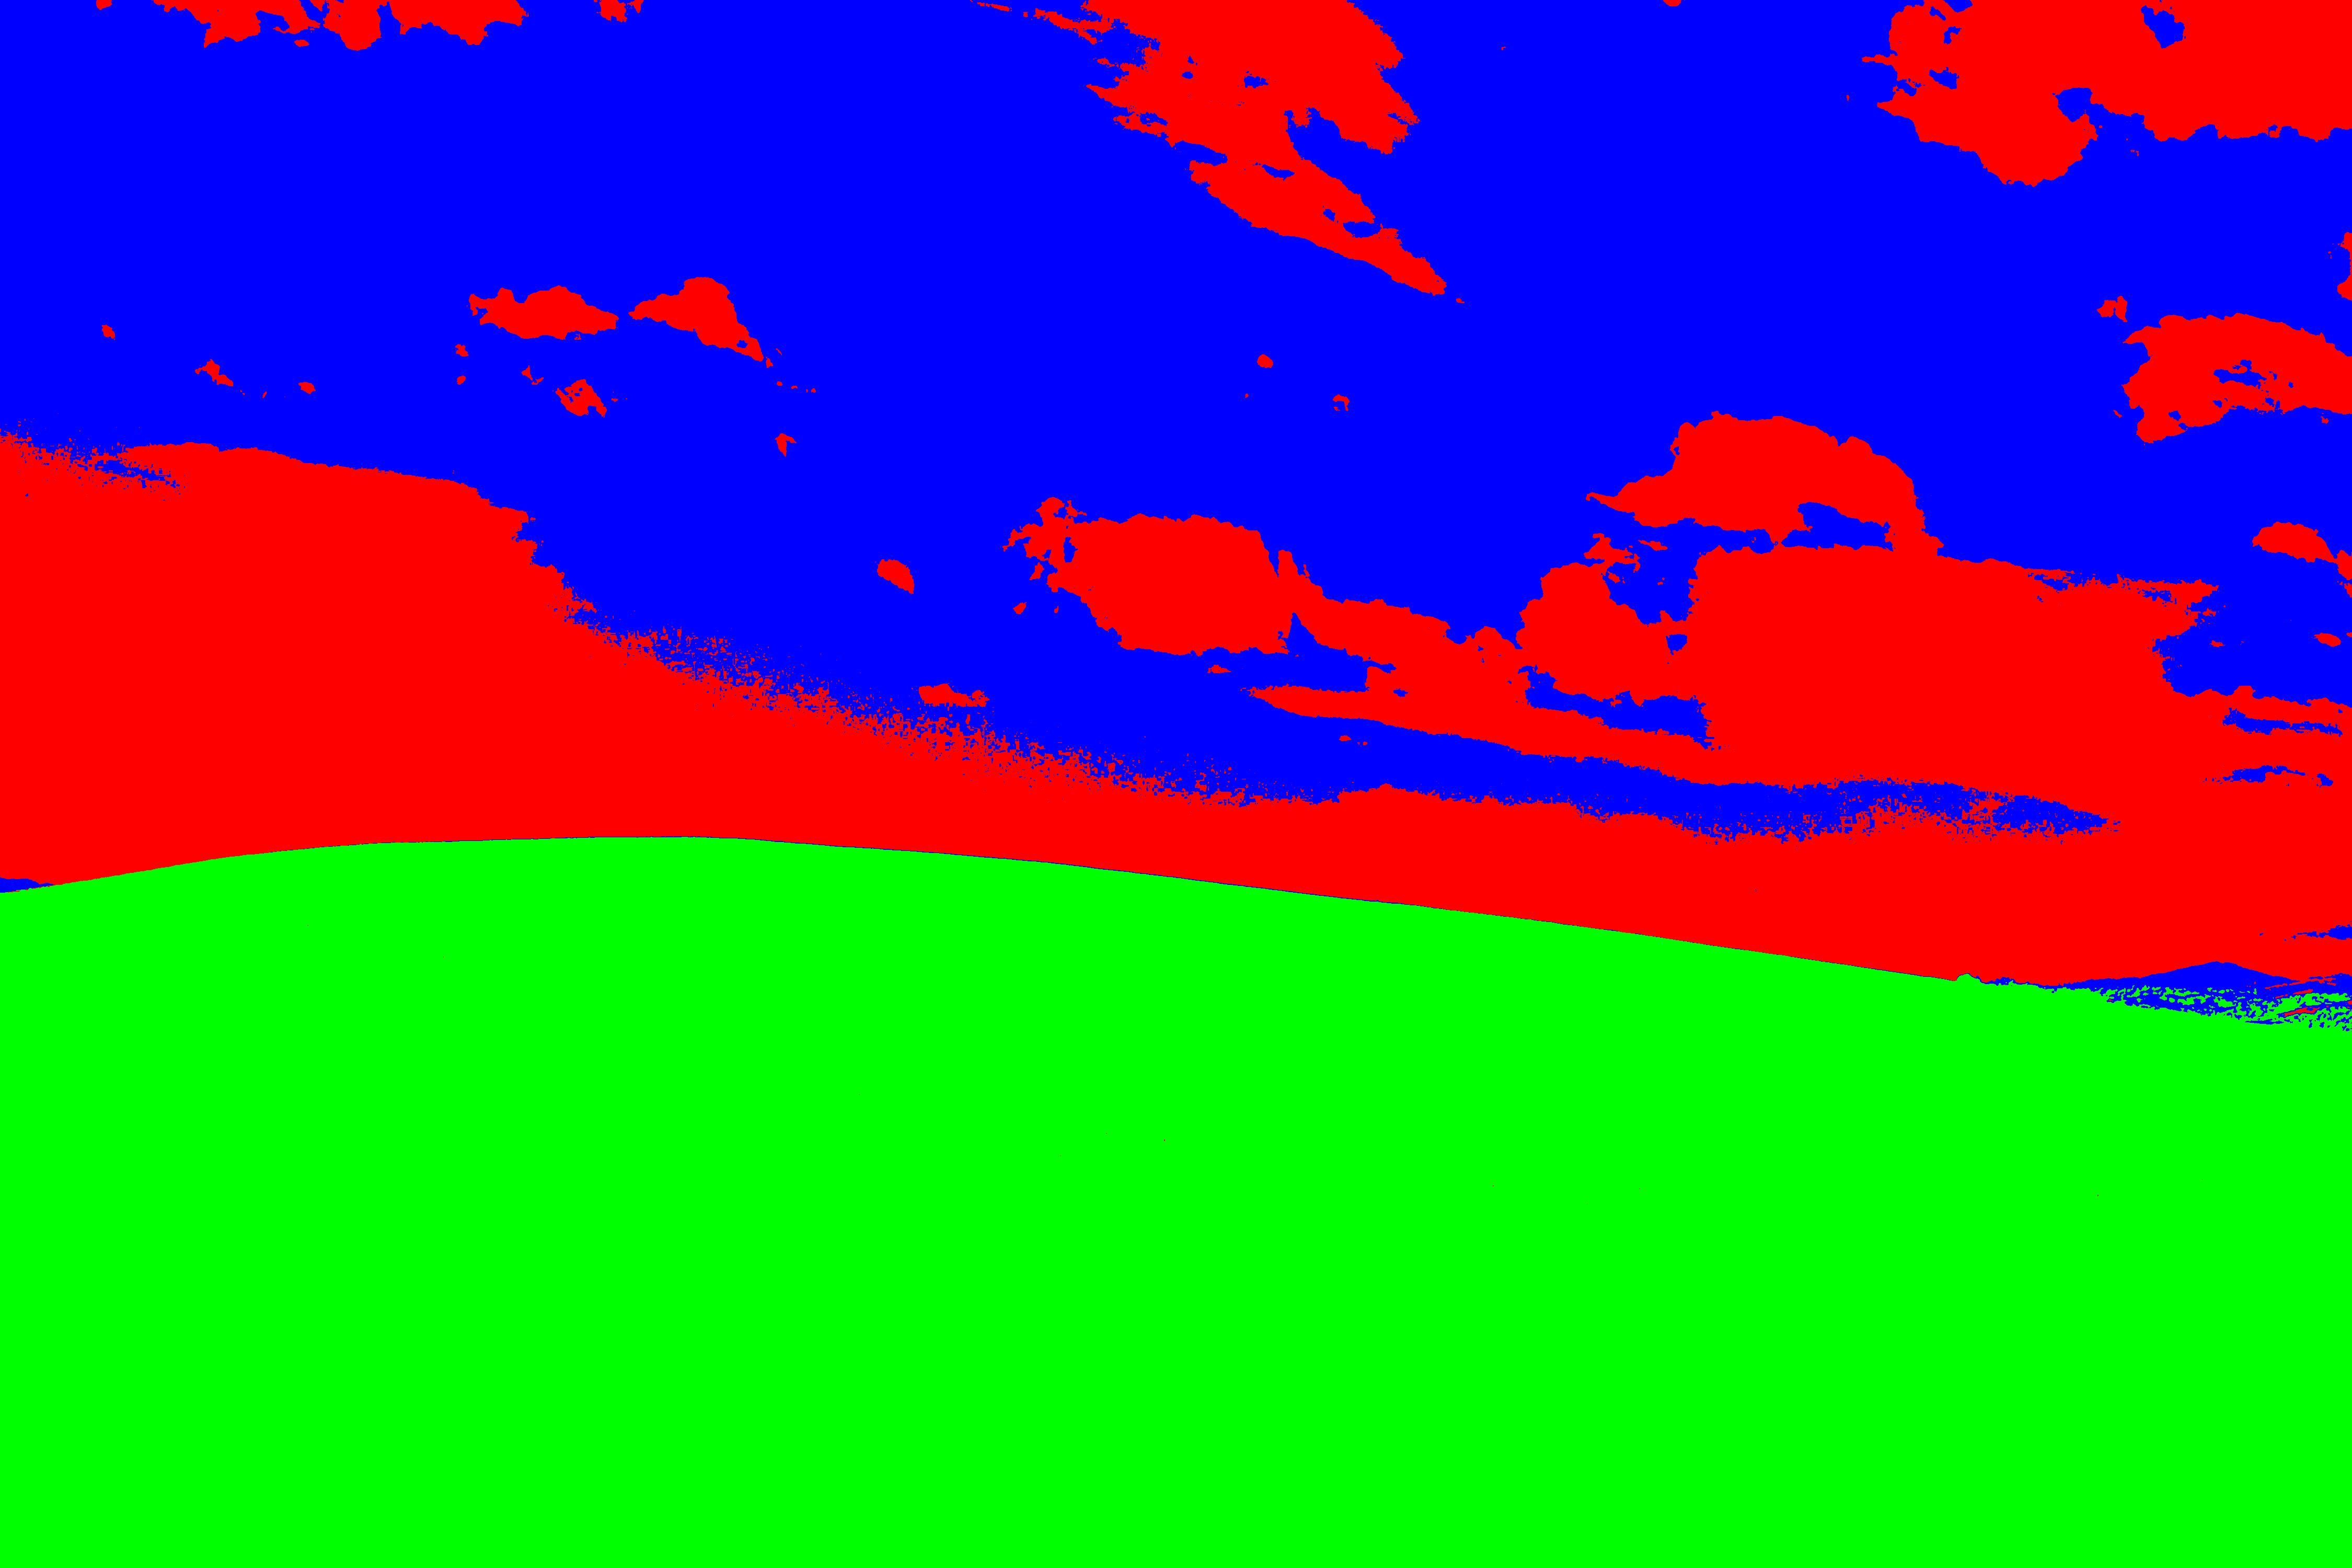
\includegraphics[height=4cm, width=5.5cm]{segmented_image_kmeans1}\\
		\end{tabular}
		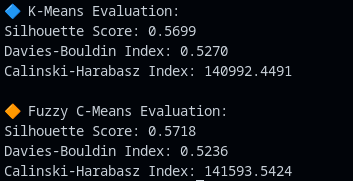
\includegraphics[height=2cm, width=3cm]{test3}
	\end{center}
\end{frame}

\begin{frame}{سوال؟؟}

\begin{enumerate}
	\item 
هر دو الگوریتم بیان شده نقاطی را به صورت رندوم برای تعیین محل اولیه خوشه ها(مراکز خوشه ها) استفاده می کنن. آیا راهی برای بهبود مقدار دهی اولیه مراکز خوشه ها وجود داره ؟
	\item 
آیا این الگوریتم کاملا یک الگوریتم بدون نظارت هستش یا نه؟
	\item
آیا راهی وجود دارد که بتوانیم با توجه به حجم داده ای که داریم پارامتر فازی ساز \lr{m} مناسب رو پیدا کنیم ؟ و آیا این مقدار می تواند به صورت اتوماتیک با توجه به حجم داده تنظیم شود؟
	\item 
چرا هر دو الگوریتم بیان شده در حال حاضر منسوخ شده اند؟

چه الگوریتم هایی در حال حاضر برای خوشه بندی استفاده میشوند.
\end{enumerate}
\end{frame}
	
	
\end{document}